\documentclass[12pt,addpoints,answers]{repaso}
\grado{1}
\nivel{Secundaria}
\cicloescolar{2024-2025}
\materia{Matemáticas 1 \normalfont \color{darkgray} \\[-0.2em] \small con adecuación curricular a Matemáticas 6$^\circ$ de Primaria}
\unidad{1, 2 y 3}
\title{Practica la Unidad}
\aprendizajes{\scriptsize%
% \item Estudio de los números.
\item Expresa oralmente la sucesión numérica hasta billones, en español y hasta donde sea posible, en su lengua materna, de manera ascendente y descendente a partir de un número natural dado. Ordena, lee y escribe números naturales de más de nueve cifras e interpreta números decimales en diferentes contextos. Identifica semejanzas y diferencias entre el sistema de numeración decimal y otros sistemas como el maya y el romano
	% \item Suma y resta, su relación como operaciones inversas.
	\item A partir de situaciones problemáticas vinculadas a diferentes contextos, suma y resta números decimales y fracciones con diferentes denominadores.
	% \item Multiplicación y división, su relación como operaciones inversas.
	\item Resuelve situaciones problemáticas vinculadas a diferentes contextos que implican dividir números decimales entre naturales. También, dividir números fraccionarios entre números naturales.
	% \item Relaciones de proporcionalidad.
	\item A partir de situaciones problemáticas de proporcionalidad vinculadas a diferentes contextos, determina valores faltantes en las que en ocasiones se conoce el valor unitario y en otras no.
	% \item Ubicación espacial.
	\item Lee, interpreta y elabora planos para comunicar la ubicación de seres vivos y objetos.
	% \item Figuras y cuerpos geométricos y sus características.
	\item Explora y reconoce las características del cilindro y cono; anticipa y comprueba desarrollos planos que permiten construirlos.
	% \item Perímetro, área y noción de volumen.
	\item Resuelve situaciones problemáticas que implican calcular el perímetro y área de figuras compuestas por triángulos y cuadriláteros. Resuelve problemas que implican construir, estimar y comparar el volumen de cuerpos y prismas rectos rectangulares mediante el conteo de cubos, y reconoce que existen diferentes cuerpos con el mismo volumen.
	% \item Organización e interpretación de datos.
	\item Interpreta información cuantitativa y cualitativa contenida en tablas, gráficas de barras y circulares para responder preguntas vinculadas a diferentes contextos; construye gráficas de barras. Genera y organiza datos, determina la moda, la media aritmética y el rango para responder preguntas vinculadas a diferentes contextos.
	% \item Nociones de probabilidad.
	\item Clasifica eventos de diversos contextos utilizando términos como seguro, imposible, probable, muy probable o poco probable que sucedan.
}
\author{Melchor Pinto, JC}
\begin{document}
\INFO
\begin{multicols}{2}
	\tableofcontents
\end{multicols}\newpage
\begin{questions}\large
	\addcontentsline{toc}{section}{Unidad 1}
	\section*{Unidad 1}


	\addcontentsline{toc}{subsection}{Sumas y Restas}
	\subsection*{Sumas y Restas}
	% \addcontentsline{toc}{subsubsection}{Sumas 1}
	% \subsubsection*{Sumas 1}
	% \addcontentsline{toc}{subsubsection}{Sumas 2}
	% \subsubsection*{Sumas 2}
	% \addcontentsline{toc}{subsubsection}{Restas 1}
	% \subsubsection*{Restas 1}
	% \addcontentsline{toc}{subsubsection}{Restas 2}
	% \subsubsection*{Restas 2}
	% \addcontentsline{toc}{subsubsection}{Resolucion de problemas}
	% \subsubsection*{Resolucion de problemas}

	\addcontentsline{toc}{subsection}{Multiplicaciones y Divisiones}
	\subsection*{Multiplicaciones y Divisiones}
	% \addcontentsline{toc}{subsubsection}{Multiplicaciones 1}
	% \subsubsection*{Multiplicaciones 1}
	% \addcontentsline{toc}{subsubsection}{Multiplicaciones 2}
	% \subsubsection*{Multiplicaciones 2}
	% \addcontentsline{toc}{subsubsection}{Divisiones 1}
	% \subsubsection*{Divisiones 1}
	% \addcontentsline{toc}{subsubsection}{Divisiones 2}
	% \subsubsection*{Divisiones 2}
	% \addcontentsline{toc}{subsubsection}{Resolucion de problemas}
	% \subsubsection*{Resolucion de problemas}

	

	\addcontentsline{toc}{subsection}{Números decimales}
	\subsection*{Números decimales}
	% \addcontentsline{toc}{subsubsection}{Posición decimal y notación desarrollada}
	% \subsubsection*{Posición decimal y notación desarrollada}
	% \addcontentsline{toc}{subsubsection}{Nombre de decimales}
	% \subsubsection*{Nombre de decimales}
\questionboxed[2]{Escribe los siguientes números

	\begin{multicols}{2}
		\begin{parts}\normalsize
			\part Catorce enteros diecinueve centésimos 	\hfill \fillin[14.19][1.2cm]
			\part Cuatro enteros once diez milésimos 		\hfill \fillin[4.0011][1.2cm]
			\part Seis enteros setenta y dos centésimos 	\hfill \fillin[6.72][1.2cm]
			\part Siete enteros novecientos tres milésimos 	\hfill \fillin[7.903][1.2cm]
			\part Seis enteros doscientos trece milésimos 	\hfill \fillin[6.213][1.2cm]
			\part Cincuenta enteros cinco décimos 			\hfill \fillin[50.5][1.2cm]
			\part Nueve enteros cuatro centésimos 			\hfill \fillin[9.04][1.2cm]
			\part Cuatro enteros setecientos doce milésimos \hfill \fillin[4.712][1.2cm]
			\part Seis mil catorce diez milésimos 			\hfill \fillin[0.6014][1.2cm]
			\part Nueve enteros once centésimos 			\hfill \fillin[9.11][1.2cm]
			\part Cuarenta enteros cuatro centésimos 		\hfill \fillin[40.04][1.2cm]
			\part Dieciocho enteros siete décimos 			\hfill \fillin[18.7][1.2cm]
			\part Veinte enteros tres décimos 				\hfill \fillin[20.3][1.2cm]
			\part Cuatro enteros ciento dos diez milésimos 	\hfill \fillin[4.0102][1.2cm]
			\part Ocho enteros trece diez milésimos 		\hfill \fillin[8.0013][1.2cm]
		\end{parts}
	\end{multicols}
}
	
	% \addcontentsline{toc}{subsubsection}{Decimales en la recta numérica}
	% \subsubsection*{Decimales en la recta numérica}

	\questionboxed[2]{Escribe en el recuadro el número decimal que representa el punto en la recta numérica de cada imagen:

		\begin{multicols}{2}
			\begin{parts}
				\part 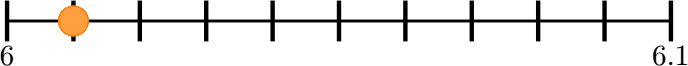
\includegraphics[width=180px]{../images/recta_num_6.01.png}  \hfill \fillin[\fbox{6.01}][0in] \\
				\part 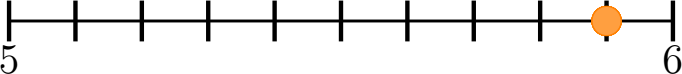
\includegraphics[width=180px]{../images/recta_num_5.9.png}   \hfill \fillin[\fbox{5.9 }][0in] \\
				\part 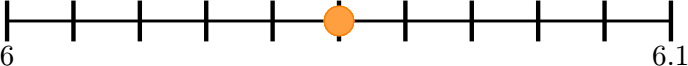
\includegraphics[width=180px]{../images/recta_num_6.05.png}  \hfill \fillin[\fbox{6.05}][0in] \\
				\part 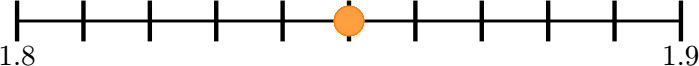
\includegraphics[width=180px]{../images/recta_num_1.85.png}  \hfill \fillin[\fbox{1.85}][0in] \\
				\part 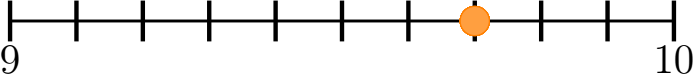
\includegraphics[width=180px]{../images/recta_num_9.7.png}   \hfill \fillin[\fbox{9.7 }][0in] \\
				\part 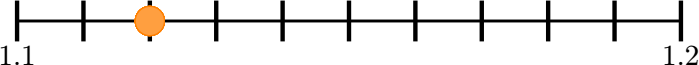
\includegraphics[width=180px]{../images/recta_num_1.12.png}  \hfill \fillin[\fbox{1.12}][0in] \\
				\part 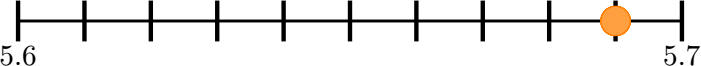
\includegraphics[width=180px]{../images/recta_num_5.69.png}  \hfill \fillin[\fbox{5.69}][0in] \\
				\part 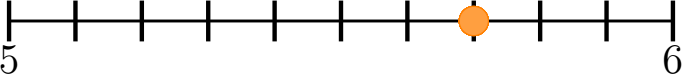
\includegraphics[width=180px]{../images/recta_num_5.7.png}   \hfill \fillin[\fbox{5.7 }][0in] \\
				\part 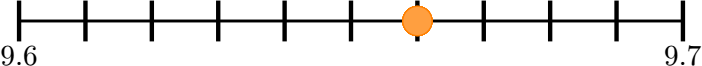
\includegraphics[width=180px]{../images/recta_num_9.66.png}  \hfill \fillin[\fbox{9.66}][0in] \\
				\part 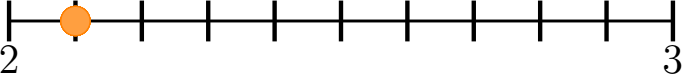
\includegraphics[width=180px]{../images/recta_num_2.1.png}   \hfill \fillin[\fbox{2.1 }][0in] \\
			\end{parts}
		\end{multicols}
	}

	% \addcontentsline{toc}{subsubsection}{Comparación de decimales}
	% \subsubsection*{Comparación de decimales}
	% \addcontentsline{toc}{subsubsection}{Redondeo de decimales}
	% \subsubsection*{Redondeo de decimales}
	

\questionboxed[2]{Señala la opción que responda correctamente a cada una de las siguientes preguntas:

	\begin{multicols}{2}
		\begin{parts}
			\part En el número 1.829, ¿qué número ocupa la posición de las centésimas?

			\begin{oneparcheckboxes}
				\choice 1 \CorrectChoice 2 \choice 6 \choice 8 \choice 9
			\end{oneparcheckboxes}

			\part En el número 2.087, ¿qué número ocupa la posición de las décimas?

			\begin{oneparcheckboxes}
				\CorrectChoice 0 \choice 2 \choice 7 \choice 8 \choice 9
			\end{oneparcheckboxes}

			\part En el número 5.928, ¿qué número ocupa la posición de las décimas?

			\begin{oneparcheckboxes}
				\choice 5 \choice 2 \choice 6 \choice 8 \CorrectChoice 9
			\end{oneparcheckboxes}

			\part En el número 3.284, ¿qué número ocupa la posición de las milésimas?

			\begin{oneparcheckboxes}
				\choice 2 \choice 3 \CorrectChoice 4  \choice 8 \choice 9
			\end{oneparcheckboxes}

			\part En el número 1.285, ¿qué número ocupa la posición de las décimas?

			\begin{oneparcheckboxes}
				\choice 1 \CorrectChoice 2 \choice 5 \choice 8 \choice 9
			\end{oneparcheckboxes}

			\part En el número 1.823, ¿qué número ocupa la posición de las milésimas?

			\begin{oneparcheckboxes}
				\choice 1 \choice 2 \CorrectChoice 3 \choice 6 \choice 8
			\end{oneparcheckboxes}
		\end{parts}
	\end{multicols}
}
	

	\addcontentsline{toc}{subsection}{Operaciones con decimales}
	\subsection*{Operaciones con decimales}
		% \addcontentsline{toc}{subsubsection}{Suma de decimales}
	% \subsubsection*{Suma de decimales}

	\questionboxed[2]{Realiza las siguientes sumas con números decimales:

		\begin{multicols}{3}
			\begin{parts}
				\part \ifprintanswers{   \opadd[hfactor=decimal,resultstyle=\color{red},carryadd=true,carrysub=false]{24.34}{13.84} }
				\else{            \opadd[hfactor=decimal,resultstyle=\color{white},carryadd=false,carrysub=false]{24.34}{13.84}\\[0.5cm]}
				\fi

				\part \ifprintanswers{   \opadd[hfactor=decimal,resultstyle=\color{red},carryadd=true,carrysub=false]{684.99}{583.82} }
				\else{           \opadd[hfactor=decimal,resultstyle=\color{white},carryadd=false,carrysub=false]{684.99}{583.82} \\[0.5cm]}
				\fi

				\part \ifprintanswers{   \opadd[hfactor=decimal,resultstyle=\color{red},carryadd=true,carrysub=false]{51.238}{34.993} }
				\else{            \opadd[hfactor=decimal,resultstyle=\color{white},carryadd=false,carrysub=false]{51.238}{34.993}\\[0.5cm] }
				\fi

				\part \ifprintanswers{   \opadd[hfactor=decimal,resultstyle=\color{red},carryadd=true,carrysub=false]{90.371}{45.392} }
				\else{            \opadd[hfactor=decimal,resultstyle=\color{white},carryadd=false,carrysub=false]{90.371}{45.392} \\[0.5cm]}
				\fi

				\part \ifprintanswers{   \opadd[hfactor=decimal,resultstyle=\color{red},carryadd=true,carrysub=false]{18.03}{7.45} }
				\else{            \opadd[hfactor=decimal,resultstyle=\color{white},carryadd=false,carrysub=false]{18.03}{7.45}\\[0.5cm] }
				\fi

				\part \ifprintanswers{   \opadd[hfactor=decimal,resultstyle=\color{red},carryadd=true,carrysub=false]{9.931}{5.198} }
				\else{           \opadd[hfactor=decimal,resultstyle=\color{white},carryadd=false,carrysub=false]{9.931}{5.198}\\[0.5cm] }
				\fi
			\end{parts}
		\end{multicols}
	}

	% \addcontentsline{toc}{subsubsection}{Resta de decimales}
	% \subsubsection*{Resta de decimales}

	\questionboxed[2]{Realiza las siguientes restas con números decimales:

		\begin{multicols}{3}
			\begin{parts}
				\part \ifprintanswers{   \opsub[hfactor=decimal,resultstyle=\color{red},carryadd=true,carrysub=true]{9.754}{3.862} }
				\else{            \opsub[hfactor=decimal,resultstyle=\color{white},carryadd=false,carrysub=false]{9.754}{3.862}\\[0.5cm]}
				\fi

				\part \ifprintanswers{   \opsub[hfactor=decimal,resultstyle=\color{red},carryadd=true,carrysub=true]{1.668}{1.464} }
				\else{            \opsub[hfactor=decimal,resultstyle=\color{white},carryadd=false,carrysub=false]{1.668}{1.464} \\[0.5cm]}
				\fi

				\part \ifprintanswers{   \opsub[hfactor=decimal,resultstyle=\color{red},carryadd=true,carrysub=true]{4.298}{3.465} }
				\else{            \opsub[hfactor=decimal,resultstyle=\color{white},carryadd=false,carrysub=false]{4.298}{3.465}\\[0.5cm] }
				\fi

				\part \ifprintanswers{   \opsub[hfactor=decimal,resultstyle=\color{red},carryadd=true,carrysub=true]{90.371}{45.392} }
				\else{            \opsub[hfactor=decimal,resultstyle=\color{white},carryadd=false,carrysub=false]{90.371}{45.392} \\[0.5cm]}
				\fi

				\part \ifprintanswers{   \opsub[hfactor=decimal,resultstyle=\color{red},carryadd=true,carrysub=true]{16.03}{6.45} }
				\else{            \opsub[hfactor=decimal,resultstyle=\color{white},carryadd=false,carrysub=false]{16.03}{6.45}\\[0.5cm] }
				\fi

				\part \ifprintanswers{   \opsub[hfactor=decimal,resultstyle=\color{red},carryadd=true,carrysub=true]{6.231}{2.188} }
				\else{            \opsub[hfactor=decimal,resultstyle=\color{white},carryadd=false,carrysub=false]{6.231}{2.188}\\[0.5cm] }
				\fi
			\end{parts}
		\end{multicols}
	}

		% \addcontentsline{toc}{subsubsection}{Multiplicación de decimales}
	% \subsubsection*{Multiplicación de decimales}
	\questionboxed[2]{Realiza las siguientes multiplicaciones con números decimales:

		\begin{multicols}{3}
			\begin{parts}
				\part \ifprintanswers{\normalsize\opmul[hfactor=decimal,resultstyle=\color{red},displayintermediary=None]{3.24}{2.52} }
				\else{\opmul[hfactor=decimal,resultstyle=\color{white},displayintermediary=None]{3.24}{2.52}}\\[2em]\fi

				\part \ifprintanswers{\normalsize\opmul[hfactor=decimal,resultstyle=\color{red},displayintermediary=all]{7.75}{3.8} }
				\else{\opmul[hfactor=decimal,resultstyle=\color{white},displayintermediary=None]{7.75}{3.8}}\\[2em]\fi

				\part \ifprintanswers{\normalsize\opmul[hfactor=decimal,resultstyle=\color{red},displayintermediary=None]{1.9}{1.2} }
				\else{\opmul[hfactor=decimal,resultstyle=\color{white},displayintermediary=None]{1.9}{1.2}}\\[2em]\fi

				\part \ifprintanswers{\normalsize\opmul[hfactor=decimal,resultstyle=\color{red},displayintermediary=all]{2.5}{2.3} }
				\else{\opmul[hfactor=decimal,resultstyle=\color{white},displayintermediary=None]{2.5}{2.3}}\\[2em]\fi

				\part \ifprintanswers{\normalsize\opmul[hfactor=decimal,resultstyle=\color{red},displayintermediary=all]{23.4}{8.5} }
				\else{\opmul[hfactor=decimal,resultstyle=\color{white},displayintermediary=None]{23.4}{8.5}}\\[2em]\fi

				\part \ifprintanswers{\normalsize\opmul[hfactor=decimal,resultstyle=\color{red},displayintermediary=all]{5.3}{1.6} }
				\else{\opmul[hfactor=decimal,resultstyle=\color{white},displayintermediary=None]{5.3}{1.6}}\\[2em]\fi
			\end{parts}
		\end{multicols}
	}


	% \addcontentsline{toc}{subsubsection}{División de decimales}
	% \subsubsection*{División de decimales}
	% \addcontentsline{toc}{subsubsection}{Resolución de problemas}
	% \subsubsection*{Resolución de problemas}


	\addcontentsline{toc}{section}{Unidad 2}
	\section*{Unidad 2}

	\addcontentsline{toc}{subsection}{Introducción a las fracciones}
	\subsection*{Introducción a las fracciones}
	

	% \addcontentsline{toc}{subsubsection}{Clasificación de fracciones}
	% \subsubsection*{Clasificación de fracciones}

	\questionboxed[2]{Clasifica las siguientes fracciones en propias, impropias o mixtas:

	\begin{multicols}{4}
		\begin{parts}
			\part $\dfrac{5}{6}$   \fillin[Propia][1in]     \\[0.5em]
			\part $5\dfrac{5}{11}$ \fillin[Mixta][1in]      \\[0.5em]
			\part $\dfrac{13}{12}$   \fillin[Impropia][1in] \\[0.5em]
			\part $1\dfrac{2}{15}$  \fillin[Mixta][1in]     \\[0.5em]
			\part $\dfrac{42}{43}$   \fillin[Propia][1in]   \\[0.5em]
			\part $\dfrac{16}{9}$   \fillin[Impropia][1in]  \\[0.5em]
			\part $\dfrac{7}{3}$   \fillin[Impropia][1in]   \\[0.5em]
			\part $3\dfrac{2}{9}$  \fillin[Mixta][1in]      \\[0.5em]
			\part $\dfrac{3}{2}$   \fillin[Impropia][1in]   \\[0.5em]
			\part $1\dfrac{2}{3}$  \fillin[Mixta][1in]      \\[0.5em]
			\part $\dfrac{7}{8}$   \fillin[Propia][1in]     \\[0.5em]
			\part $\dfrac{6}{5}$   \fillin[Impropia][1in]   \\[0.5em]
		\end{parts}
	\end{multicols}
}

	% \addcontentsline{toc}{subsubsection}{Representación de fracciones}
	% \subsubsection*{Representación de fracciones}

	\questionboxed[2]{Escribe sobre la línea la fracción que representa cada imagen:

		\begin{multicols}{4}
			\begin{parts}
				\part 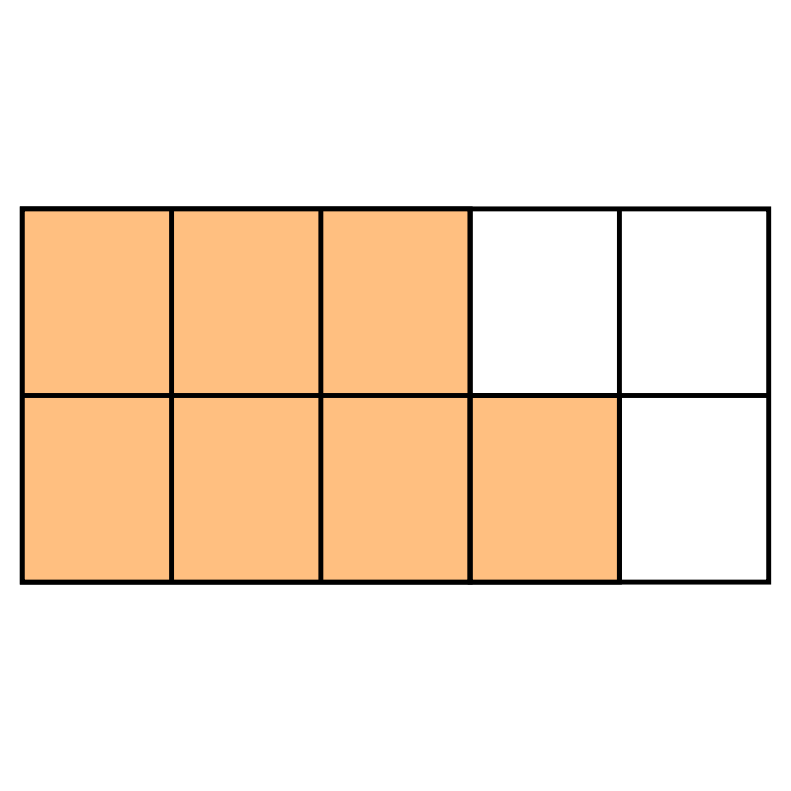
\includegraphics[width=50px]{../images/imagen_frac_5prim_7|10.png} \fillin[\fbox{$\dfrac{7}{10}$}][0in] \\[-0.5em]
				\part 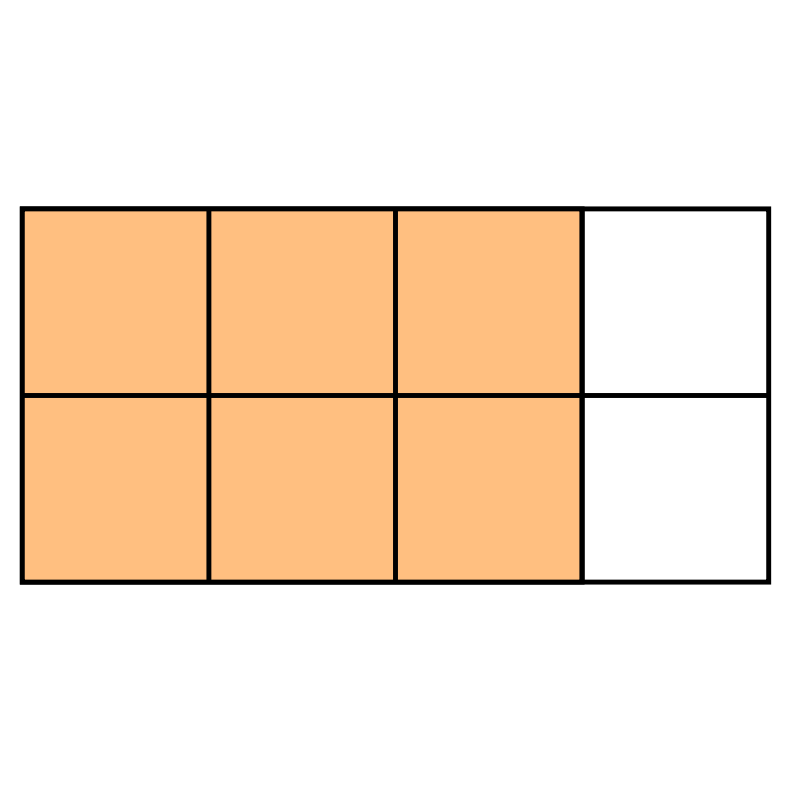
\includegraphics[width=50px]{../images/imagen_frac_5prim_6|8.png} \fillin[\fbox{$\dfrac{6}{8}$}][0in] \\[-0.5em]
				\part 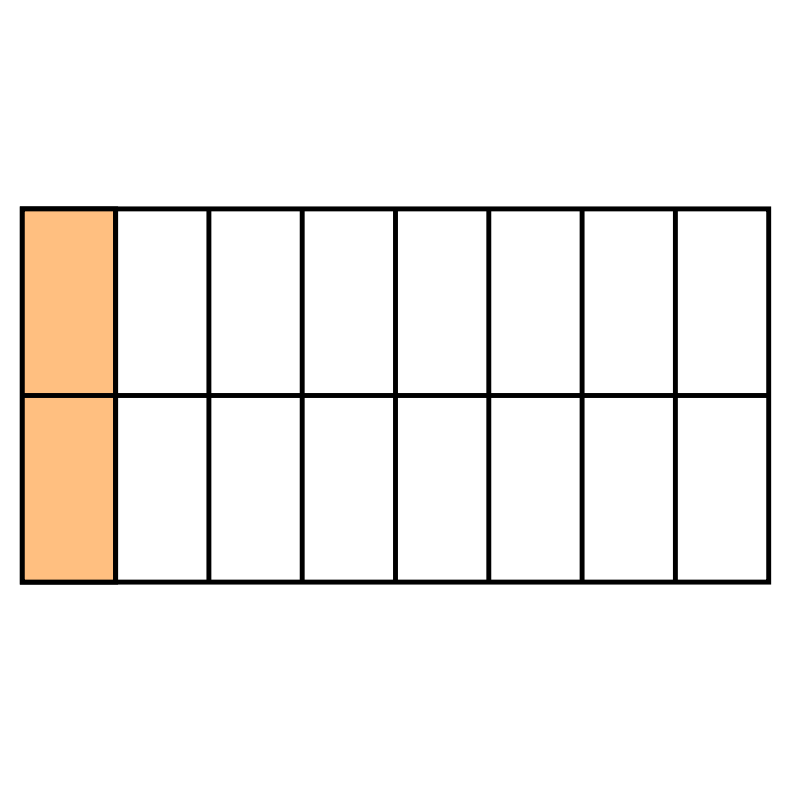
\includegraphics[width=50px]{../images/imagen_frac_5prim_2|16.png} \fillin[\fbox{$\dfrac{2}{16}$}][0in] \\[-0.5em]
				\part 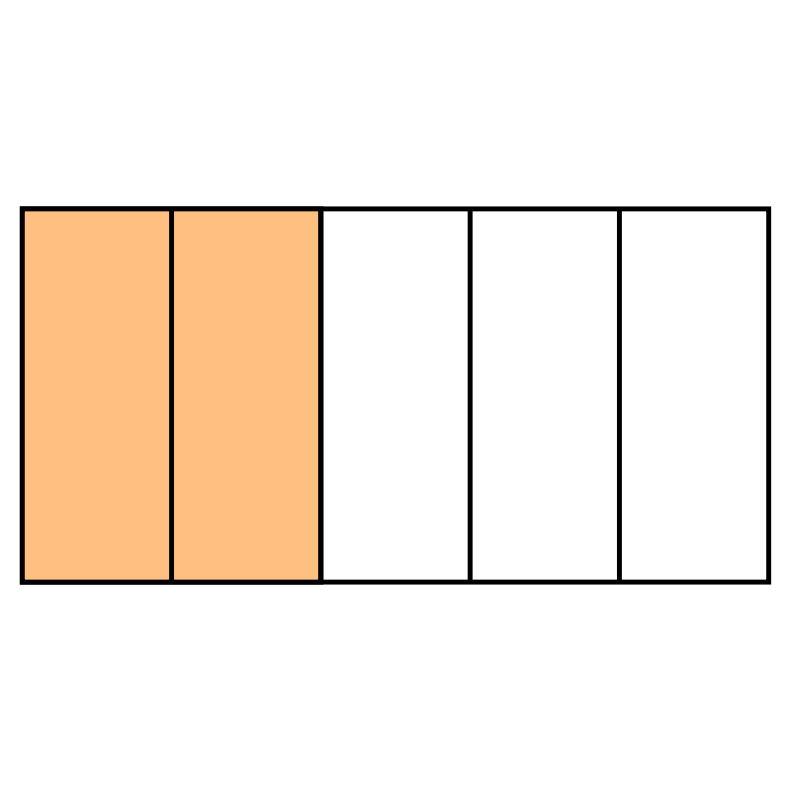
\includegraphics[width=50px]{../images/imagen_frac_5prim_2|5.png} \fillin[\fbox{$\dfrac{2}{5}$}][0in] \\[-0.5em]
				\part 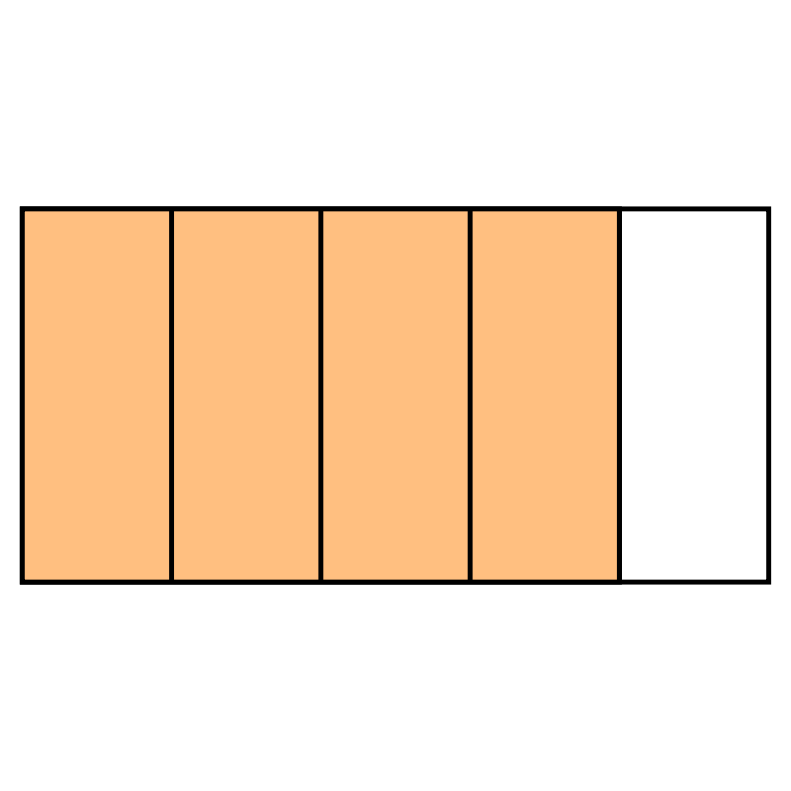
\includegraphics[width=50px]{../images/imagen_frac_5prim_4|5.png} \fillin[\fbox{$\dfrac{4}{5}$}][0in] \\[-0.5em]
				\part 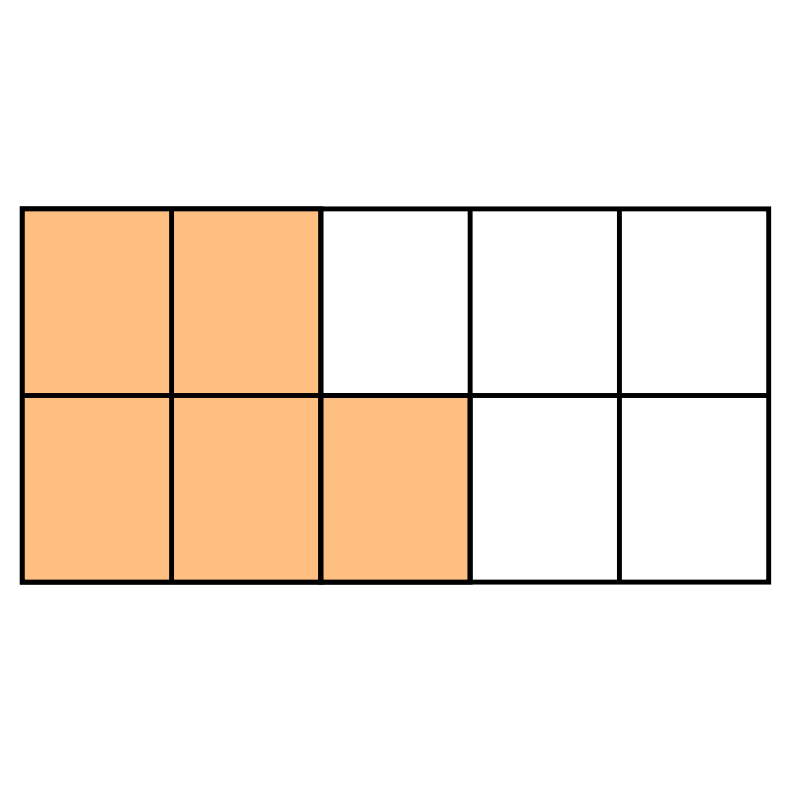
\includegraphics[width=50px]{../images/imagen_frac_5prim_5|10.png} \fillin[\fbox{$\dfrac{5}{10}$}][0in] \\[-0.5em]
				\part 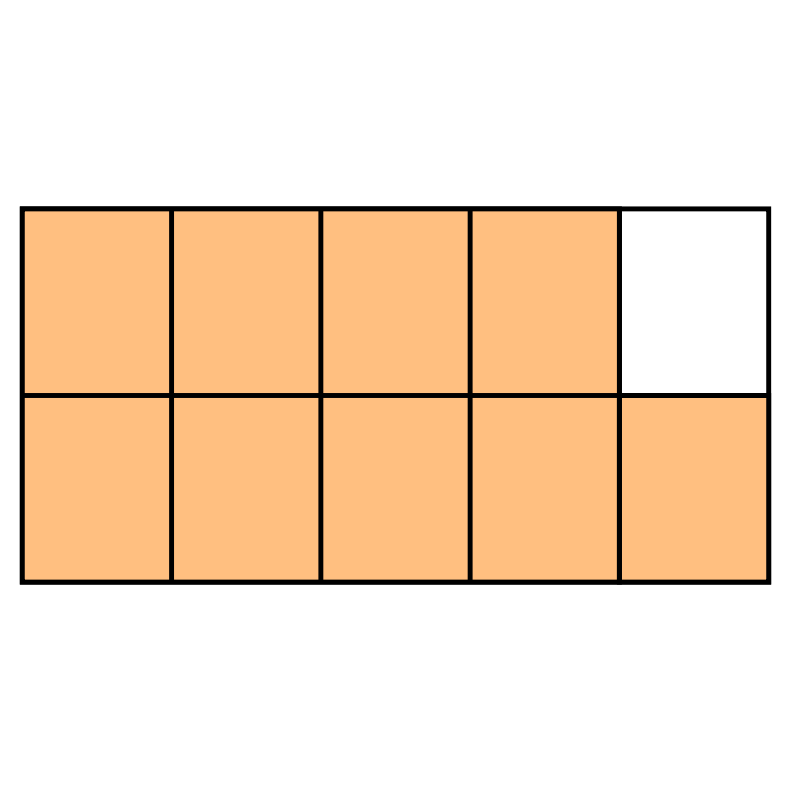
\includegraphics[width=50px]{../images/imagen_frac_5prim_9|10.png} \fillin[\fbox{$\dfrac{9}{10}$}][0in] \\[-0.5em]
				\part 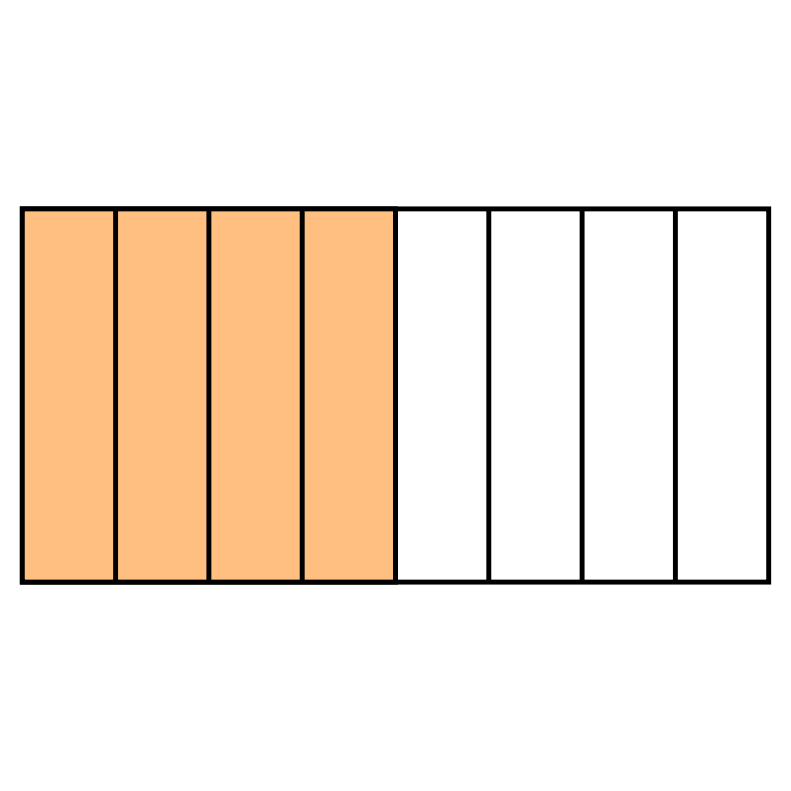
\includegraphics[width=50px]{../images/imagen_frac_5prim_4|8.png} \fillin[\fbox{$\dfrac{4}{8}$}][0in] \\[-0.5em]
				\part 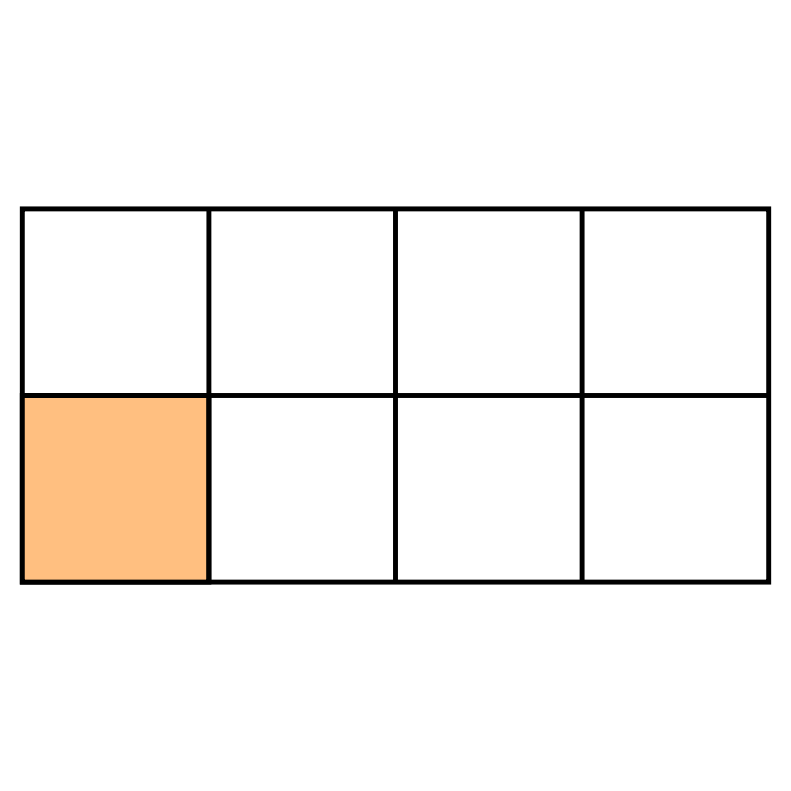
\includegraphics[width=50px]{../images/imagen_frac_5prim_1|8.png} \fillin[\fbox{$\dfrac{1}{8}$}][0in] \\[-0.5em]
				\part 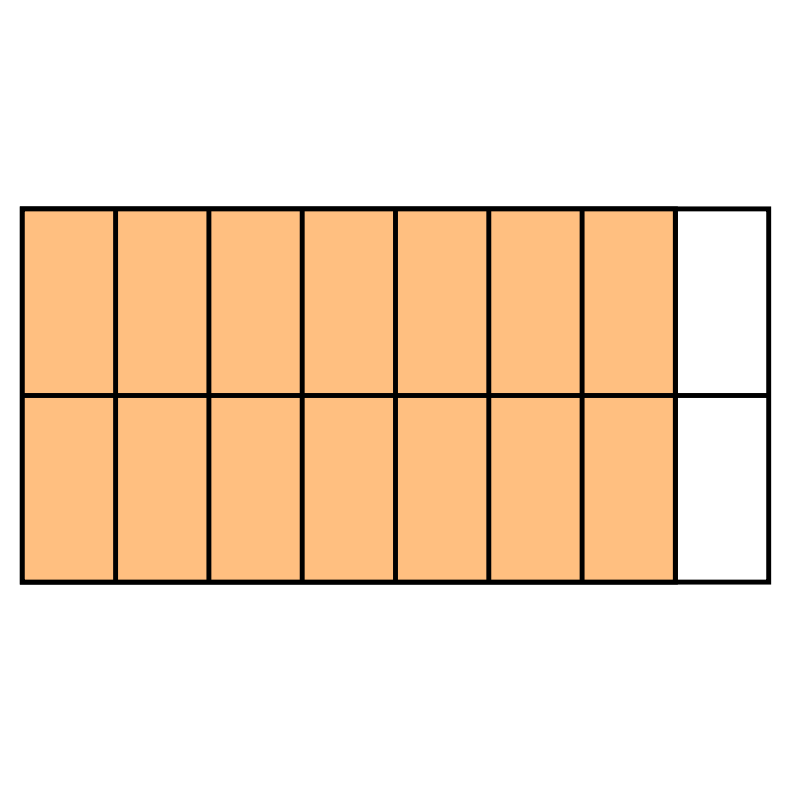
\includegraphics[width=50px]{../images/imagen_frac_5prim_14|16.png} \fillin[\fbox{$\dfrac{14}{16}$}][0in] \\[-0.5em]
				\part 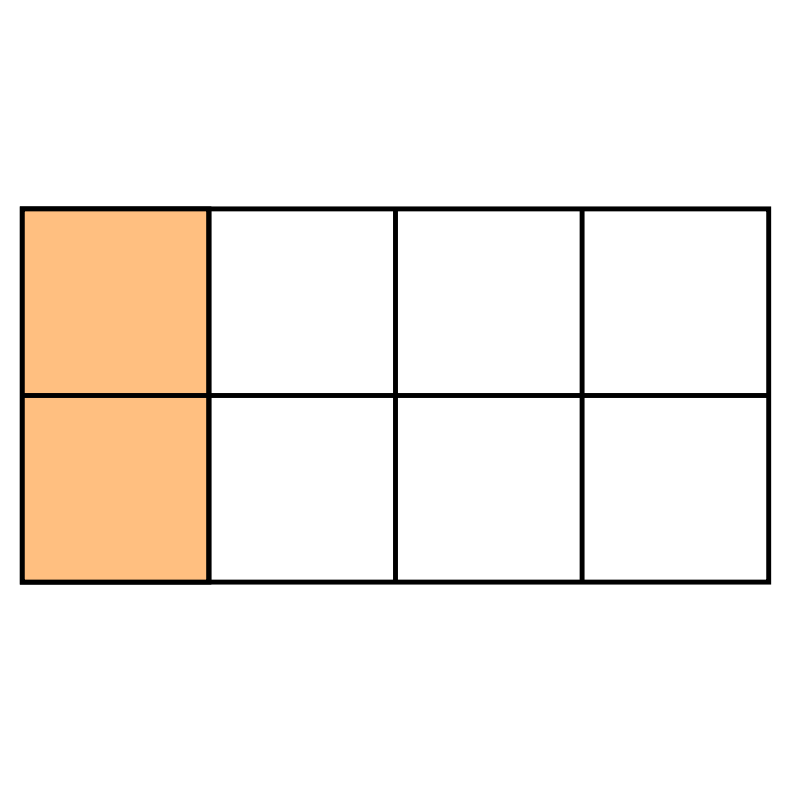
\includegraphics[width=50px]{../images/imagen_frac_5prim_2|8.png} \fillin[\fbox{$\dfrac{2}{8}$}][0in] \\[-0.5em]
				\part 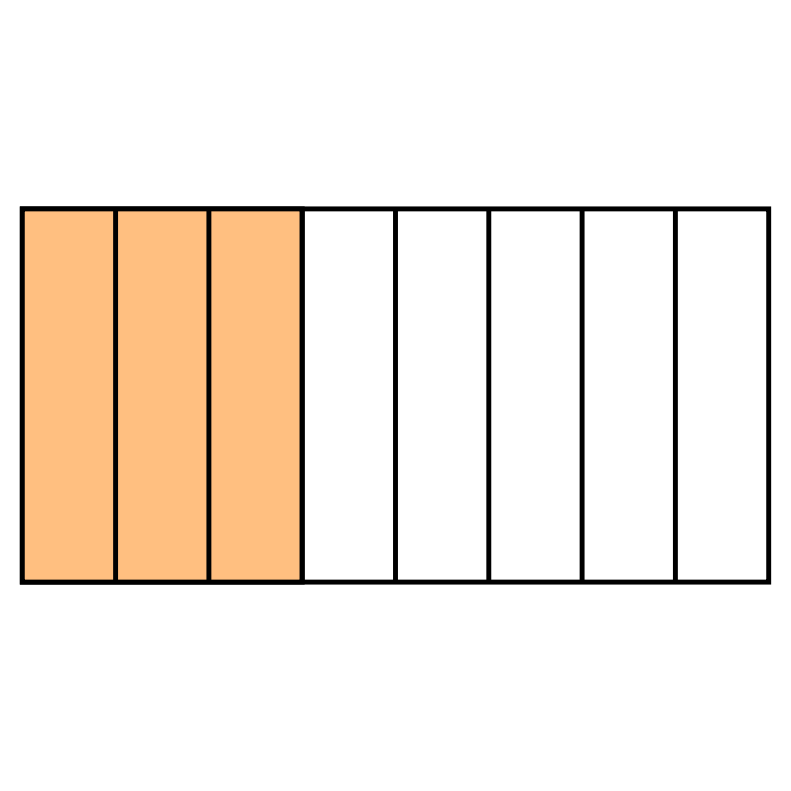
\includegraphics[width=50px]{../images/imagen_frac_5prim_3|8.png} \fillin[\fbox{$\dfrac{3}{8}$}][0in] \\[-0.5em]
				\part 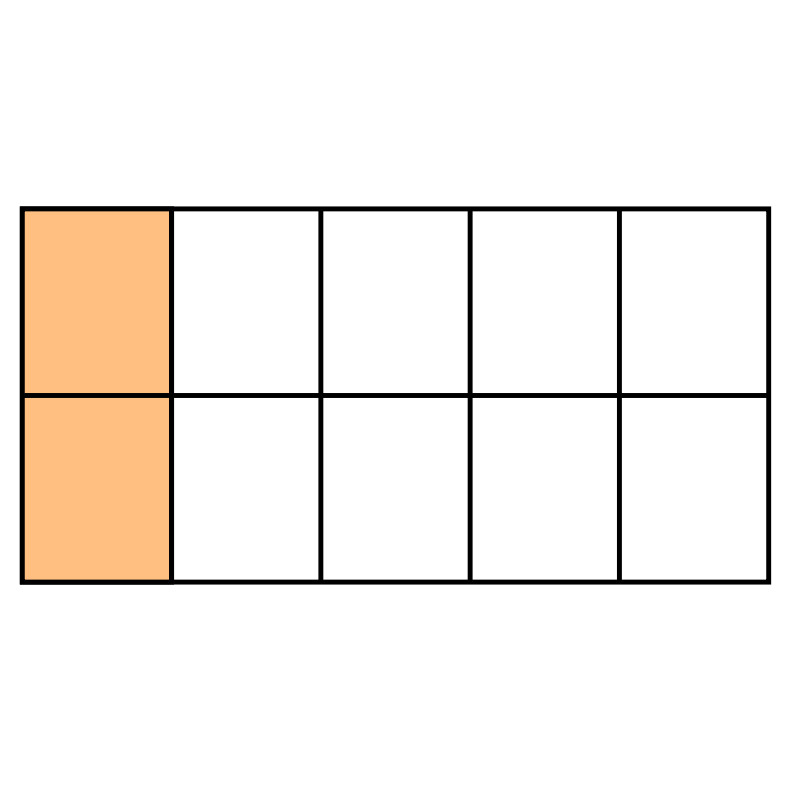
\includegraphics[width=50px]{../images/imagen_frac_5prim_2|10.png} \fillin[\fbox{$\dfrac{2}{10}$}][0in] \\[-0.5em]
				\part 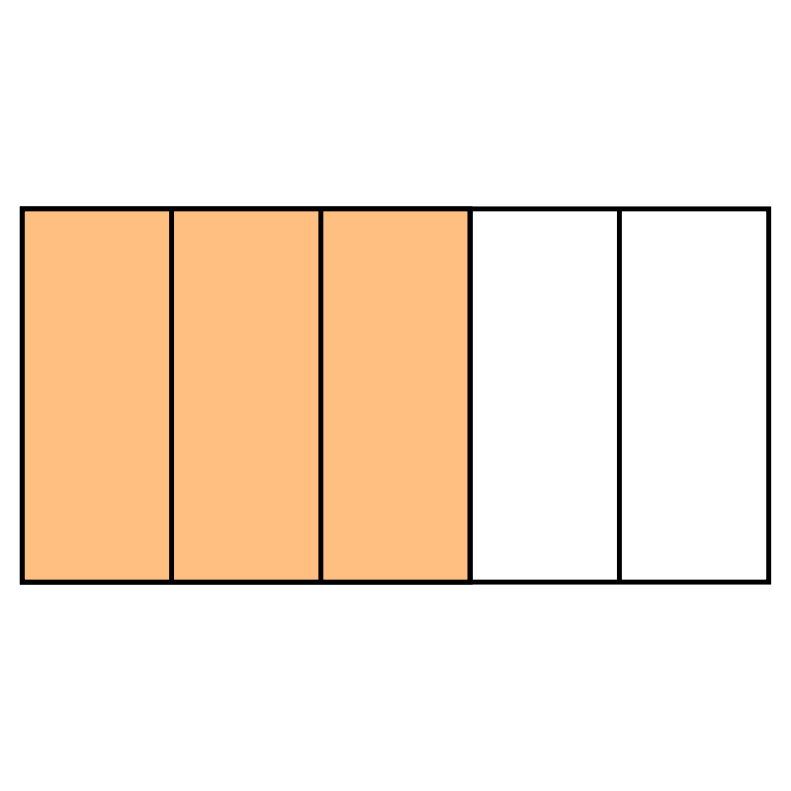
\includegraphics[width=50px]{../images/imagen_frac_5prim_3|5.png} \fillin[\fbox{$\dfrac{3}{5}$}][0in] \\[-0.5em]
				\part 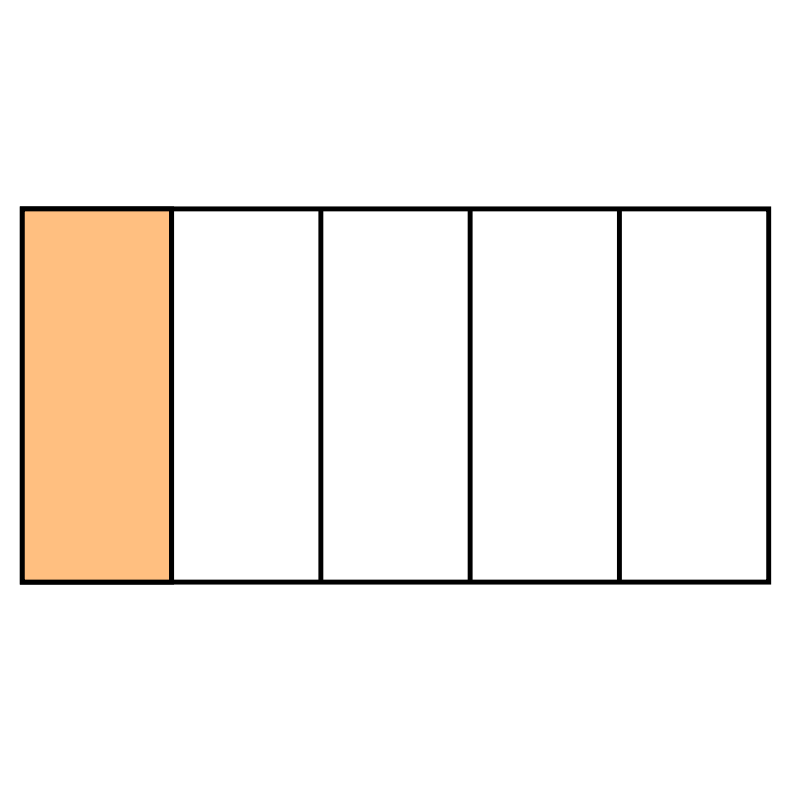
\includegraphics[width=50px]{../images/imagen_frac_5prim_1|5.png} \fillin[\fbox{$\dfrac{1}{5}$}][0in] \\[-0.5em]
				\part 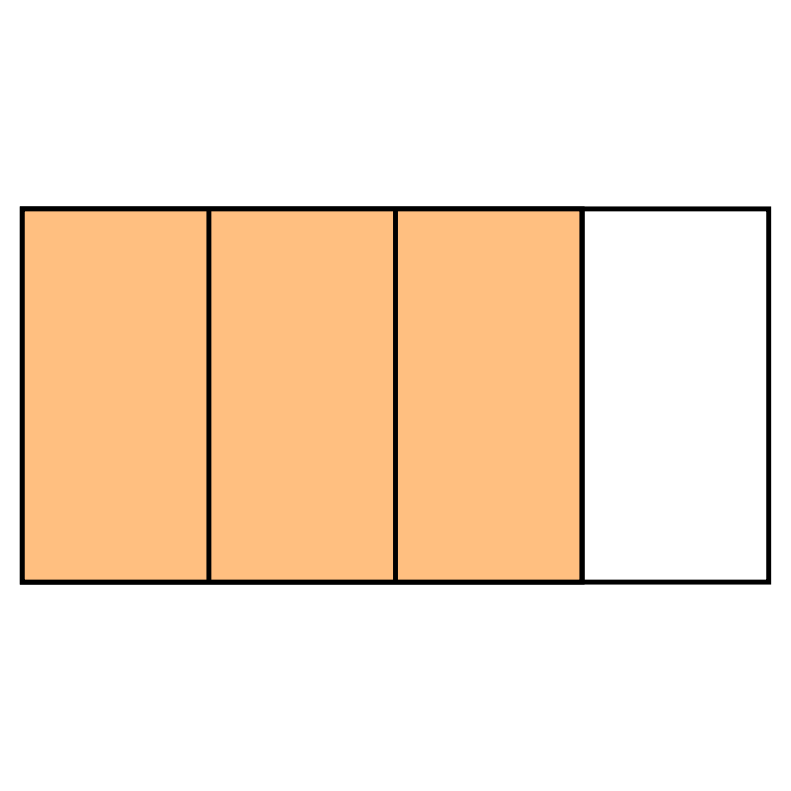
\includegraphics[width=50px]{../images/imagen_frac_5prim_3|4.png} \fillin[\fbox{$\dfrac{3}{4}$}][0in] \\[-0.5em]


			\end{parts}
		\end{multicols}
	}
	% \addcontentsline{toc}{subsubsection}{Nombre de fracciones}
	% \subsubsection*{Nombre de fracciones}

	\questionboxed[2]{Escribe la fracción que corresponda en cada inciso:

		\begin{parts}
			\part ¿Cómo se escribe numéricamente la fracción \textbf{siete catorceavos}?    \fillin[$\dfrac{7}{14}$][0in]
			\part ¿Cómo se escribe numéricamente la fracción \textbf{ocho onceavos}?   \fillin[$\dfrac{8}{11}$][0in]
			\part ¿Cómo se escribe numéricamente la fracción \textbf{doce séptimos}?    \fillin[$\dfrac{12}{7}$][0in]
			\part ¿Cómo se escribe numéricamente la fracción \textbf{nueve treceavos}?     \fillin[$\dfrac{9}{13}$][0in]
		\end{parts}
	}

	% \addcontentsline{toc}{subsubsection}{Fracciones en la recta numérica}
	% \subsubsection*{Fracciones en la recta numérica}
	
	\questionboxed[2]{Escribe la fracción que representa el punto en la recta numérica de cada imagen:

		\begin{multicols}{2}
			\begin{parts}
				\part 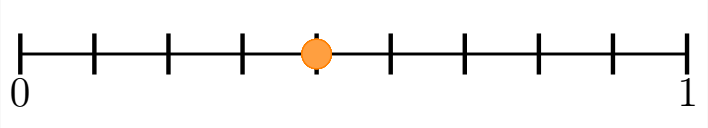
\includegraphics[width=180px]{../images/recta_num_frac4|9.png}   \hfill \fillin[\fbox{$\dfrac{ 4}{9 }$}][0in] \\
				\part 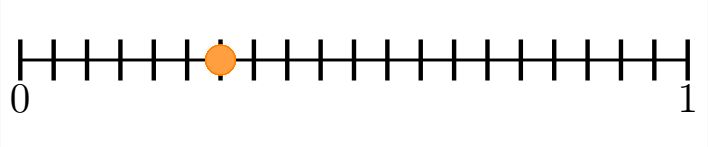
\includegraphics[width=180px]{../images/recta_num_frac6|20.png}  \hfill \fillin[\fbox{$\dfrac{ 6}{20}$}][0in] \\
				\part 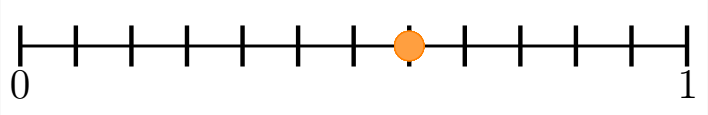
\includegraphics[width=180px]{../images/recta_num_frac7|12.png}  \hfill \fillin[\fbox{$\dfrac{ 7}{12}$}][0in] \\
				\part 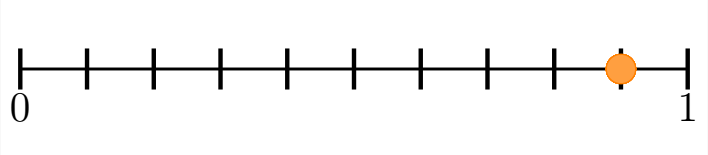
\includegraphics[width=180px]{../images/recta_num_frac9|10.png}  \hfill \fillin[\fbox{$\dfrac{ 9}{10}$}][0in] \\
				\part 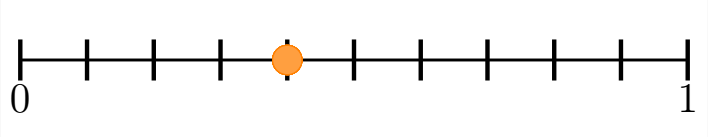
\includegraphics[width=180px]{../images/recta_num_frac4|10.png}  \hfill \fillin[\fbox{$\dfrac{ 4}{10}$}][0in] \\
				\part 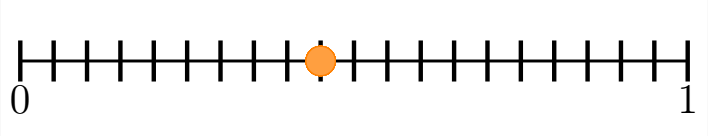
\includegraphics[width=180px]{../images/recta_num_frac9|20.png}  \hfill \fillin[\fbox{$\dfrac{ 9}{20}$}][0in] \\
				\part 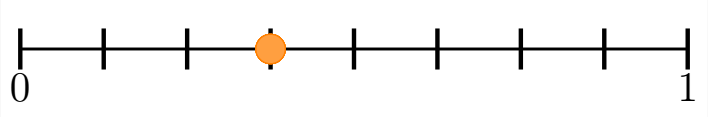
\includegraphics[width=180px]{../images/recta_num_frac3|8.png}   \hfill \fillin[\fbox{$\dfrac{ 3}{8 }$}][0in] \\
				\part 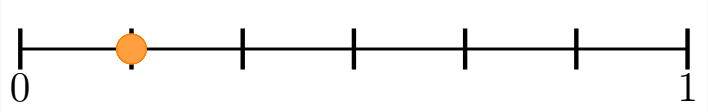
\includegraphics[width=180px]{../images/recta_num_frac1|6.png}   \hfill \fillin[\fbox{$\dfrac{ 1}{6 }$}][0in] \\
				\part 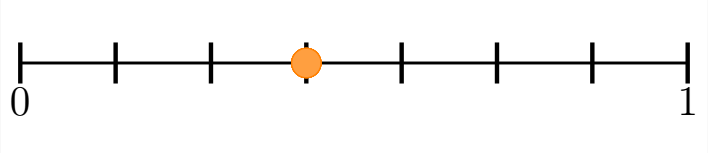
\includegraphics[width=180px]{../images/recta_num_frac3|7.png}   \hfill \fillin[\fbox{$\dfrac{ 3}{7 }$}][0in] \\
				\part 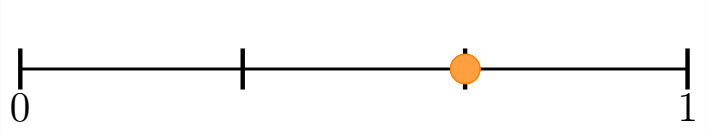
\includegraphics[width=180px]{../images/recta_num_frac2|3.png}   \hfill \fillin[\fbox{$\dfrac{ 2}{3 }$}][0in] \\
			\end{parts}
		\end{multicols}
	}
	% \addcontentsline{toc}{subsubsection}{Conversión de fracciones}
	% \subsubsection*{Conversión de fracciones}
	% \subsection*{Conversión de fracciones}

	\questionboxed[2]{Convierte la siguientes fracciones mixtas a impropias y viseversa:

		\begin{multicols}{3}
			\begin{parts}
				\part $4\dfrac{2}{3}= $  \fillin[$\dfrac{14}{3}$][0in]\\[0.5em]
				\part $\dfrac{13}{3}= $  \fillin[$4\dfrac{1}{3}$][0in]\\[0.5em]
				\part $2\dfrac{3}{10}= $ \fillin[$\dfrac{23}{10}$][0in]\\[0.5em]
				\part $\dfrac{43}{10}= $ \fillin[$4\dfrac{3}{10}$][0in]\\[0.5em]
				\part $5\dfrac{1}{5}= $  \fillin[$\dfrac{26}{5}$][0in]\\[0.5em]
				\part $\dfrac{51}{5}= $  \fillin[$10\dfrac{1}{5}$][0in]\\[0.5em]
			\end{parts}
		\end{multicols}
	}

	\addcontentsline{toc}{subsection}{Simplificación de fracciones}
	\subsection*{Simplificación de fracciones}
	% \addcontentsline{toc}{subsubsection}{Comparación de fracciones}
	% \subsubsection*{Comparación de fracciones}
	% \addcontentsline{toc}{subsubsection}{Fracciones equivalentes}
	% \subsubsection*{Fracciones equivalentes}

	\questionboxed[2]{Indica si las siguientes fracciones son equivalentes o no:

		\begin{multicols}{2}
			\begin{parts}

				\part $\dfrac{1}{2}=\dfrac{4}{6}$\qquad
				\begin{oneparcheckboxes}
					\choice Sí
					\CorrectChoice No
				\end{oneparcheckboxes}

				\part $\dfrac{4}{5}=\dfrac{8}{10}$\qquad
				\begin{oneparcheckboxes}
					\CorrectChoice Sí
					\choice No
				\end{oneparcheckboxes}

				\part $\dfrac{1}{8}=\dfrac{4}{16}$\qquad
				\begin{oneparcheckboxes}
					\choice Sí
					\CorrectChoice No
				\end{oneparcheckboxes}

				\part $\dfrac{1}{5}=\dfrac{5}{10}$\qquad
				\begin{oneparcheckboxes}
					\choice Sí
					\CorrectChoice No
				\end{oneparcheckboxes}

				\part $\dfrac{1}{10}=\dfrac{3}{30}$\qquad
				\begin{oneparcheckboxes}
					\CorrectChoice Sí
					\choice No
				\end{oneparcheckboxes}

				\part $\dfrac{1}{4}=\dfrac{2}{4}$\qquad
				\begin{oneparcheckboxes}
					\choice Sí
					\CorrectChoice No
				\end{oneparcheckboxes}

				\part $\dfrac{1}{5}=\dfrac{10}{25}$\qquad
				\begin{oneparcheckboxes}
					\choice Sí
					\CorrectChoice No
				\end{oneparcheckboxes}

				\part $\dfrac{3}{2}=\dfrac{12}{8}$\qquad
				\begin{oneparcheckboxes}
					\CorrectChoice Sí
					\choice No
				\end{oneparcheckboxes}

				\part $\dfrac{3}{6}=\dfrac{1}{3}$\qquad
				\begin{oneparcheckboxes}
					\choice Sí
					\CorrectChoice No
				\end{oneparcheckboxes}

				\part $\dfrac{18}{12}=\dfrac{9}{4}$\qquad
				\begin{oneparcheckboxes}
					\choice Sí
					\CorrectChoice No
				\end{oneparcheckboxes}
			\end{parts}
		\end{multicols}
	}
	% \addcontentsline{toc}{subsubsection}{Mínimo Común Múltiplo}
	% \subsubsection*{Mínimo Común Múltiplo}
	% \addcontentsline{toc}{subsubsection}{Máxico Común Divisor}
	% \subsubsection*{Máxico Común Divisor}
	% \addcontentsline{toc}{subsubsection}{Simplificación de fracciones}
	% \subsubsection*{Simplificación de fracciones}
	\questionboxed[2]{Simplifica a su mínima expresión las siguientes fracciones usando el máximo común divisor:

		\begin{multicols}{5}
			\begin{parts}
				\part $\dfrac{12}{48}= $  \fillin[$\dfrac{1}{4}$][0in]\\[0.5em]
				\part $\dfrac{6}{24}= $  \fillin[$\dfrac{1}{4}$][0in]\\[0.5em]
				\part $\dfrac{16}{36}= $  \fillin[$\dfrac{4}{9}$][0in]\\[0.5em]
				\part $\dfrac{4}{40}= $  \fillin[$\dfrac{1}{10}$][0in]\\[0.5em]
				\part $\dfrac{4}{20}= $  \fillin[$\dfrac{1}{5}$][0in]\\[0.5em]
				\part $\dfrac{2}{30}= $  \fillin[$\dfrac{1}{15}$][0in]\\[0.5em]
				\part $\dfrac{6}{36}= $  \fillin[$\dfrac{1}{6}$][0in]\\[0.5em]
				\part $\dfrac{5}{25}= $  \fillin[$\dfrac{1}{5}$][0in]\\[0.5em]
				\part $\dfrac{6}{30}= $  \fillin[$\dfrac{1}{5}$][0in]\\[0.5em]
				\part $\dfrac{2}{12}= $  \fillin[$\dfrac{1}{6}$][0in]\\[0.5em]
				\part $\dfrac{4}{16}= $  \fillin[$\dfrac{1}{4}$][0in]\\[0.5em]
				\part $\dfrac{15}{20}= $  \fillin[$\dfrac{3}{4}$][0in]\\[0.5em]
				\part $\dfrac{5}{50}= $  \fillin[$\dfrac{1}{10}$][0in]\\[0.5em]
				\part $\dfrac{6}{10}= $  \fillin[$\dfrac{3}{5}$][0in]\\[0.5em]
				\part $\dfrac{3}{18}= $  \fillin[$\dfrac{1}{6}$][0in]\\[0.5em]
			\end{parts}
		\end{multicols}
	}

	\addcontentsline{toc}{subsection}{Suma y resta de fracciones}
	\subsection*{Suma y resta de fracciones}



	\questionboxed[4]{Realiza las siguientes operaciones de suma y resta de fracciones:

	\begin{multicols}{3}
		\begin{parts}
			\part $\dfrac{3}{5}+\dfrac{4}{5}=$ \fillin[$\dfrac{7}{5} = 1\dfrac{2}{5}$][0in] \\[1em]
			\part $\dfrac{3}{10}+\dfrac{4}{5}=$ \fillin[$\dfrac{11}{10} = 1\dfrac{1}{10}$][0in] \\[1em]
			\part $\dfrac{9}{10}+\dfrac{2}{3}=$ \fillin[$1\dfrac{17}{30}$][0in] \\[1em]
			\part $\dfrac{13}{6}-\dfrac{5}{6}=$ \fillin[$\dfrac{8}{6}=\dfrac{4}{3}$][0in] \\[1em]
			\part $1\dfrac{1}{2}+1\dfrac{2}{3}=$ \fillin[$3\dfrac{1}{6}$][0in] \\[1em]
			\part $\dfrac{3}{4}-\dfrac{2}{5}=$ \fillin[$\dfrac{7}{20}$][0in] \\[1em]
			\part $\dfrac{5}{6}+\dfrac{1}{12}=$ \fillin[$\dfrac{11}{12}$][0in] \\[1em]
			\part $\dfrac{12}{7}-\dfrac{5}{7}=$ \fillin[$\dfrac{7}{7}=1$][0in] \\[1em]
			\part $\dfrac{2}{3}-\dfrac{2}{5}=$ \fillin[$\dfrac{4}{15}$][0in] \\[1em]
			\part $2\dfrac{1}{2}-1\dfrac{1}{3}=$ \fillin[$1\dfrac{1}{6}$][0in] \\[1em]
			\part $\dfrac{1}{3}-\dfrac{1}{4}=$ \fillin[$\dfrac{1}{12}$][0in] \\[1em]
			\part $1\dfrac{1}{8}+1\dfrac{7}{8}=$ \fillin[$2\dfrac{8}{8} = 3$][0in] \\[1em]
			\part $\dfrac{3}{8}+\dfrac{7}{10}=$ \fillin[$\dfrac{43}{40} = 1\dfrac{3}{40}$][0in] \\[1em]
			\part $\dfrac{3}{4}-\dfrac{1}{8}=$ \fillin[$\dfrac{5}{8}$][0in] \\[1em]
			\part $3\dfrac{3}{4}-2\dfrac{2}{3}=$ \fillin[$1\dfrac{1}{12}$][0in] \\[1em]
		\end{parts}
	\end{multicols}
}


	\addcontentsline{toc}{subsection}{Multiplicación y división de fracciones}
	\subsection*{Multiplicación y división de fracciones}
	% \addcontentsline{toc}{subsubsection}{Suma y resta con denominadores iguales}
	% \subsubsection*{Suma y resta con denominadores iguales}
	% \addcontentsline{toc}{subsubsection}{Suma y resta denominadores diferentes}
	% \subsubsection*{Suma y resta denominadores diferentes}
	% \addcontentsline{toc}{subsubsection}{Multiplicación de fracciones}
	% \subsubsection*{Multiplicación de fracciones}
	% \addcontentsline{toc}{subsubsection}{División de fracciones}
	% \subsubsection*{División de fracciones}
	% \addcontentsline{toc}{subsubsection}{Resolución de problemas}
	% \subsubsection*{Resolución de problemas}

	\questionboxed[5]{Realiza las siguientes operaciones de multiplicación y división de fracciones (Expresa tu resultadocomo una \textbf{fracción simplificada}):

		\begin{multicols}{4}
			\begin{parts}
				\part $\dfrac{7}{9}\times\dfrac{12}{17}=$ \fillin[$\dfrac{28}{51}$][0in]   \\[1em]
				\part $\dfrac{2}{7}\divisionsymbol\dfrac{2}{5}=$ \fillin[$\dfrac{5}{7}$][0in]   \\[1em]
				\part $3\times\dfrac{5}{4}=$ \fillin[$\dfrac{15}{4}$][0in]   \\[1em]
				\part $1\dfrac{1}{4}\times 4\dfrac{5}{8}=$ \fillin[$\dfrac{185}{32}$][0in]   \\[1em]
				\part $\dfrac{5}{6}\times\dfrac{4}{5}=$ \fillin[$\dfrac{2}{3}$][0in]   \\[1em]
				\part $\dfrac{4}{7}\divisionsymbol\dfrac{5}{6}=$ \fillin[$\dfrac{24}{35}$][0in]   \\[1em]
				\part $\dfrac{7}{6}\times 6=$ \fillin[$\dfrac{21}{2}$][0in]   \\[1em]
				\part $3\dfrac{1}{3}\times 2\dfrac{2}{5}=$ \fillin[$8$][0in]   \\[1em]
				\part $\dfrac{3}{7}\times\dfrac{5}{6}=$ \fillin[$\dfrac{5}{14}$][0in]   \\[1em]
				\part $\dfrac{7}{8}\divisionsymbol\dfrac{5}{4}=$ \fillin[$\dfrac{7}{10}$][0in]   \\[1em]
				\part $\dfrac{2}{5}\divisionsymbol 5=$ \fillin[$\dfrac{2}{25}$][0in]   \\[1em]
				\part $6\dfrac{1}{2}\divisionsymbol 1\dfrac{5}{7}=$ \fillin[$\dfrac{91}{24}$][0in]   \\[1em]
				\part $\dfrac{5}{8}\times\dfrac{4}{5}=$ \fillin[$\dfrac{1}{2}$][0in]   \\[1em]
				\part $\dfrac{6}{7}\divisionsymbol\dfrac{1}{3}=$ \fillin[$\dfrac{18}{7}$][0in]   \\[1em]
				\part $4\divisionsymbol\dfrac{3}{5}=$ \fillin[$\dfrac{20}{3}$][0in]   \\[1em]
				\part $2\dfrac{2}{3}\divisionsymbol 1\dfrac{3}{4}=$ \fillin[$\dfrac{32}{21}$][0in]   \\[1em]
			\end{parts}
		\end{multicols}
	}

	\addcontentsline{toc}{subsection}{Decimales y porcentajes}
	\subsection*{Decimales y porcentajes}

	% \addcontentsline{toc}{subsubsection}{Porcentajes a decimal}
	% \subsubsection*{Porcentajes a decimal}
	\questionboxed[2]{Escribe los siguientes porcentajes como números decimales:

	\begin{multicols}{4}
		\begin{parts}
			\part $14\%=$ \fillin[\fbox{0.14}][0cm] \\
			\part $73\%=$ \fillin[\fbox{0.73}][0cm] \\
			\part $15\%=$ \fillin[\fbox{0.15}][0cm] \\
			\part $85\%=$ \fillin[\fbox{0.85}][0cm] \\
			\part $91\%=$ \fillin[\fbox{0.91}][0cm] \\
			\part $19\%=$ \fillin[\fbox{0.19}][0cm] \\
			\part $ 9\%=$ \fillin[\fbox{0.09}][0cm] \\
			\part $42\%=$ \fillin[\fbox{0.42}][0cm] \\
			\part $25\%=$ \fillin[\fbox{0.25}][0cm] \\
			\part $ 3\%=$ \fillin[\fbox{0.03}][0cm] \\
			\part $ 8\%=$ \fillin[\fbox{0.08}][0cm] \\
			\part $ 2\%=$ \fillin[\fbox{0.02}][0cm] \\
		\end{parts}
	\end{multicols}
}

	% \addcontentsline{toc}{subsubsection}{Decimales a porcentajes}
	% \subsubsection*{Decimales a porcentajes}


	\questionboxed[4]{Escribe el porcentaje que representa cada número decimal:

		\begin{multicols}{2}
			\begin{parts}
				\part $1.44=$ \fillin[$144\%$][0in]
				\part $0.092=$ \fillin[$9.2\%$][0in]
				\part $0.0005=$ \fillin[$0.05\%$][0in]
				\part $5.5=$ \fillin[$550\%$][0in]
				\part $0.33=$ \fillin[$33\%$][0in]
				\part $0.209=$ \fillin[$20.9\%$][0in]
			\end{parts}
		\end{multicols}
	}


\questionboxed[2]{Calcula los porentajes de los siguientes números:

		\begin{multicols}{2}
			\begin{parts}
				\part ¿Cuál es el 80\% de 660?   \hfill \fillin[\fbox{528}][0cm]
				\part ¿Cuál es el 20\% de 50?    \hfill \fillin[\fbox{10}][0cm]
				\part ¿Cuál es el 50\% de 862?   \hfill \fillin[\fbox{431}][0cm]
				\part ¿Cuál es el 30\% de 300?   \hfill \fillin[\fbox{90}][0cm]
				\part ¿Cuál es el 20\% de 415?   \hfill \fillin[\fbox{83}][0cm]
				\part ¿Cuál es el 12\% de 338?   \hfill \fillin[\fbox{40.56}][0cm]
				\part ¿Cuál es el 15\% de 711?   \hfill \fillin[\fbox{106.65}][0cm]
				\part ¿Cuál es el 80\% de 1260?  \hfill \fillin[\fbox{1008}][0cm]
			\end{parts}
		\end{multicols}
	}

	\questionboxed[10]{Resuelve los siguientes problemas:

	\begin{parts}
			\part El costo de una camisa es de \$800 pesos, si se les hace un descuento del 20\%, ¿cuánto pagaré en total por la camisa?
			
			\begin{solutionbox}{2cm}
				\[\$800\times 20\%=\$160\]
				\[\$800-\$160=\$640\]
			\end{solutionbox}

			\part El 24\% de los habitantes de un pueblo tienen menos de 30 años. ¿Cuántos habitantes tiene el pueblo si hay 120 jóvenes menores de 30 años?
		
			\begin{solutionbox}{2cm}
				\[\dfrac{120\times 100\%}{24\%}=500\]
			\end{solutionbox}
		\end{parts}
	}

	% \addcontentsline{toc}{subsubsection}{Operaciones con múltiplos de 10}
	% \subsubsection*{Operaciones con múltiplos de 10}
	% \addcontentsline{toc}{subsubsection}{Conversión de fracciones a decimales}
	% \subsubsection*{Conversión de fracciones a decimales}

	\questionboxed[2]{Convierte las siguientes fracciones a decimal:

		\begin{multicols}{5}
			\begin{parts}
				\part $\dfrac{2}{9} =$   \fillin[\fbox{$0.\overline{2}$}][0cm]\\
				\part $\dfrac{1}{4} =$   \fillin[\fbox{$0.25$}][0cm]\\
				\part $\dfrac{2}{3} =$   \fillin[\fbox{$0.\overline{6}$}][0cm]\\
				\part $\dfrac{7}{8} =$   \fillin[\fbox{$0.875$}][0cm]\\
				\part $\dfrac{1}{9} =$   \fillin[\fbox{$0.\overline{1}$}][0cm]\\
				\part $\dfrac{6}{8} =$   \fillin[\fbox{$0.75$}][0cm]\\
				\part $\dfrac{7}{20}=$   \fillin[\fbox{$0.35$}][0cm]\\
				\part $\dfrac{5}{8} =$   \fillin[\fbox{$0.625$}][0cm]\\
				\part $\dfrac{2}{10}=$   \fillin[\fbox{$0.2$}][0cm]\\
				\part $\dfrac{5}{6} =$   \fillin[\fbox{$0.8\overline{3}$}][0cm]\\
			\end{parts}
		\end{multicols}
	}

	% \addcontentsline{toc}{subsubsection}{Conversión de decimales a fracciones}
	% \subsubsection*{Conversión de decimales a fracciones}

	\questionboxed[2]{Convierte los siguientes números decimales a una fracción simplificada a su mínima expresión:

	\begin{multicols}{4}
		\begin{parts}
			\part $0.248=$ \fillin[\fbox{$\dfrac{31}{125}$}][0cm]
			\part $0.46=$  \fillin[\fbox{$\dfrac{23}{50}$}][0cm]
			\part $0.24=$  \fillin[\fbox{$\dfrac{6}{25}$}][0cm]
			\part $0.9=$   \fillin[\fbox{$\dfrac{9}{10}$}][0cm]
			\part $0.115=$ \fillin[\fbox{$\dfrac{23}{200}$}][0cm]
			\part $0.66=$  \fillin[\fbox{$\dfrac{33}{50}$}][0cm]
			\part $0.56=$  \fillin[\fbox{$\dfrac{14}{25}$}][0cm]
			\part $0.58=$  \fillin[\fbox{$\dfrac{29}{50}$}][0cm]
		\end{parts}
	\end{multicols}
}


	\addcontentsline{toc}{section}{Unidad 3}
	\section*{Unidad 3}

	\addcontentsline{toc}{subsection}{Círculo}
	\subsection*{Círculo}
	% \addcontentsline{toc}{subsubsection}{Diámetro de un círculo}
	% \subsubsection*{Diámetro de un círculo}
	% \addcontentsline{toc}{subsubsection}{Radio de un círculo}
	% \subsubsection*{Radio de un círculo}

	\questionboxed[2]{Contesta las siguientes preguntas:

		\begin{multicols}{2}
			\begin{parts}
				\part ¿Cuál es el diámetro de un círculo que tiene un radio de 21.98?

				\begin{solutionbox}{1cm}
					\fillin[43.96][0cm]
				\end{solutionbox}

				\part ¿Cuál es el diámetro de un círculo que tiene un radio de 39.21?

				\begin{solutionbox}{1cm}
					\fillin[78.42][0cm]
				\end{solutionbox}

				\part ¿Cuál es el diámetro de un círculo que tiene un radio de 6.7?

				\begin{solutionbox}{1cm}
					\fillin[13.4][0cm]
				\end{solutionbox}

				\part ¿Cuál es el radio de un círculo que tiene un diámetro de 88.28?

				\begin{solutionbox}{1cm}
					\fillin[44.19][0cm]
				\end{solutionbox}

			\end{parts}
		\end{multicols}
	}

	% \addcontentsline{toc}{subsubsection}{Perímetro}
	% \subsubsection*{Perímetro}
	% \addcontentsline{toc}{subsubsection}{Área}
	% \subsubsection*{Área}

	\questionboxed[2]{Calcula el perímetro y área de los siguientes círculos:

		\begin{multicols}{3}
			\begin{parts}

				\part 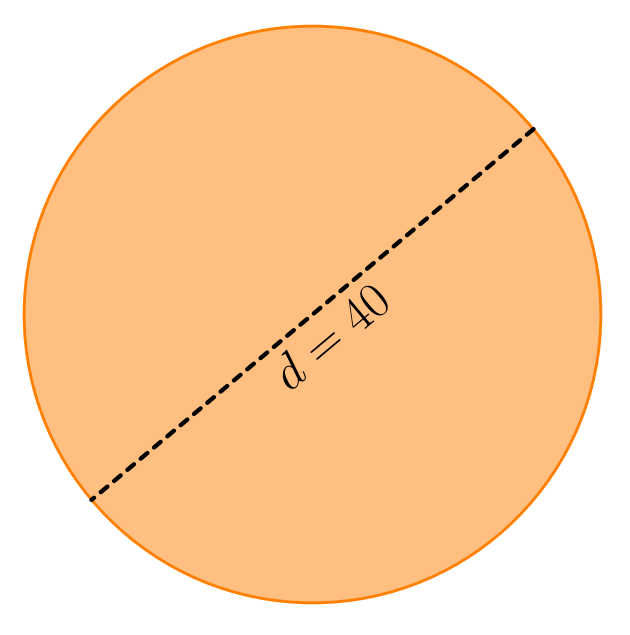
\includegraphics[width=0.8\linewidth]{../images/circulo01.png}\\
				\small Perímetro: \fillin[62.8][0.3in]  Área: \fillin[1256][0.3in]

				\begin{solutionbox}{1.2cm}\footnotesize
					% $P=8\pi=8(3.14)=25.12$ \\
					% $A=\pi(4)^2=3.14(4)^2=50.24$
				\end{solutionbox}

				\part 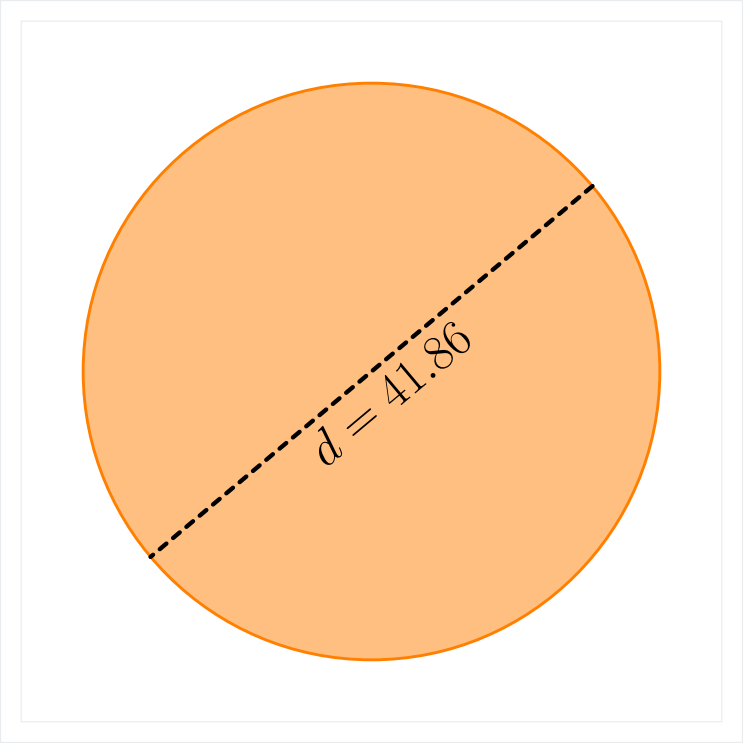
\includegraphics[width=0.8\linewidth]{../images/circulo02.png}\\
				\small Perímetro: \fillin[131.51][0.3in]  Área: \fillin[1376.22][0.3in]

				\begin{solutionbox}{1.2cm}\footnotesize
					% $P=2\pi r=2(3.14)(9.3)=58.4$ \\
					% $A=\pi r^2=3.14(9.3)^2=271.57$
				\end{solutionbox}

				\part 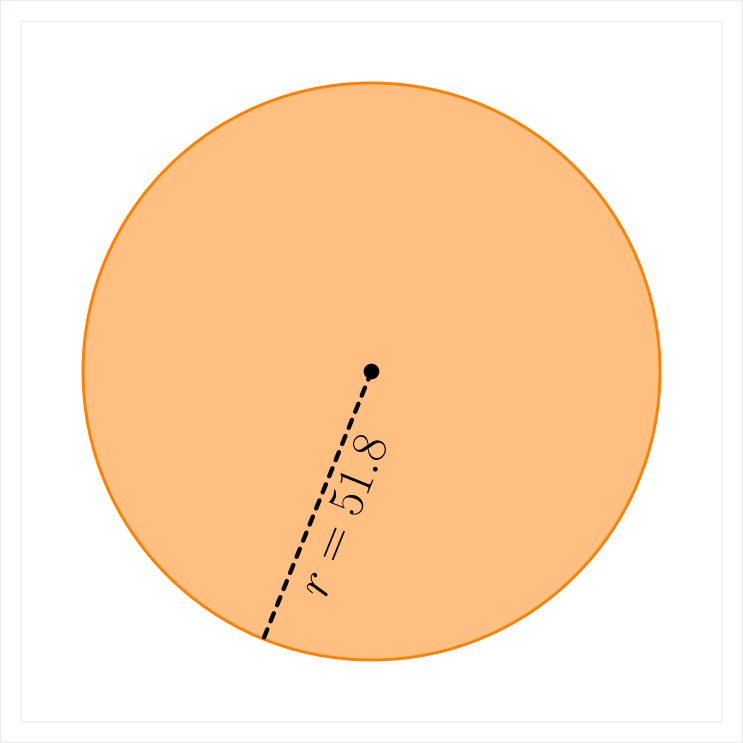
\includegraphics[width=0.8\linewidth]{../images/circulo03.png}\\
				\small Perímetro: \fillin[325.47][0.3in]  Área: \fillin[8429.65][0.3in]

				\begin{solutionbox}{1.2cm}\footnotesize
					% $P=2\pi r=2(3.14)(12)=75.36$ \\
					% $A=\pi r^2=3.14(12)^2=452.16$
				\end{solutionbox}

				\part 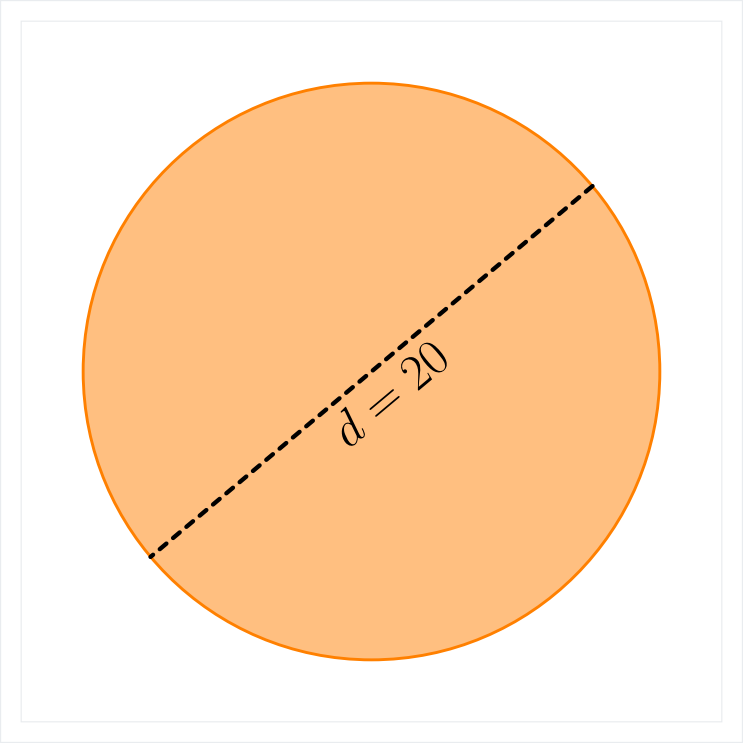
\includegraphics[width=0.8\linewidth]{../images/circulo04.png}\\
				\small Perímetro: \fillin[62.8][0.3in]  Área: \fillin[314][0.3in]

				\begin{solutionbox}{1.2cm}\footnotesize
					% $P=8\pi=8(3.14)=25.12$ \\
					% $A=\pi(4)^2=3.14(4)^2=50.24$
				\end{solutionbox}

				\part 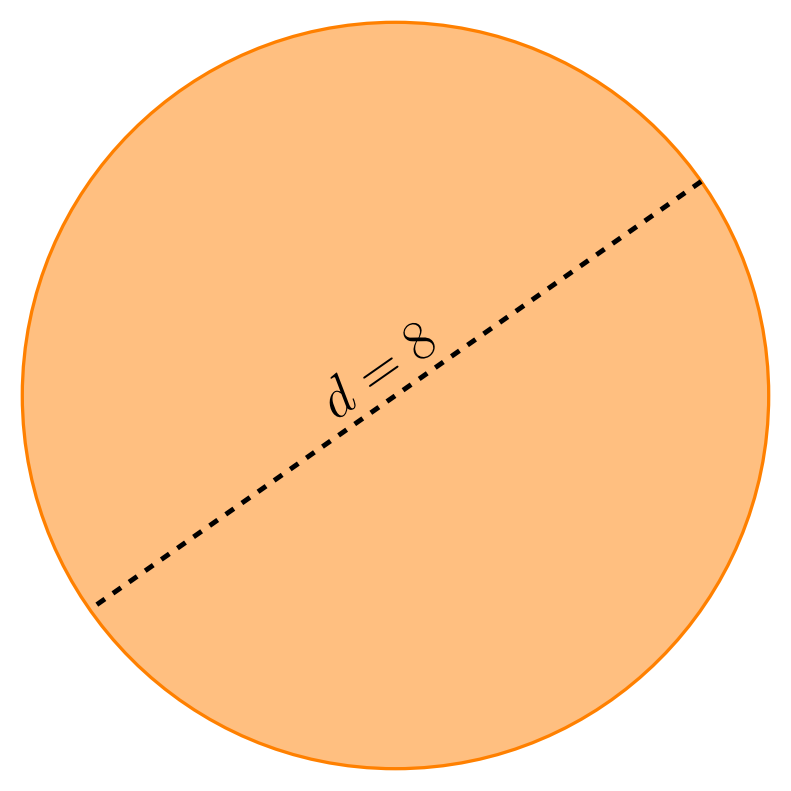
\includegraphics[width=0.8\linewidth]{../images/circulo05.png}\\
				\small Perímetro: \fillin[25.12][0.3in]  Área: \fillin[50.24][0.3in]

				\begin{solutionbox}{1.2cm}\footnotesize
					% $P=2\pi r=2(3.14)(9.3)=58.4$ \\
					% $A=\pi r^2=3.14(9.3)^2=271.57$
				\end{solutionbox}

				\part 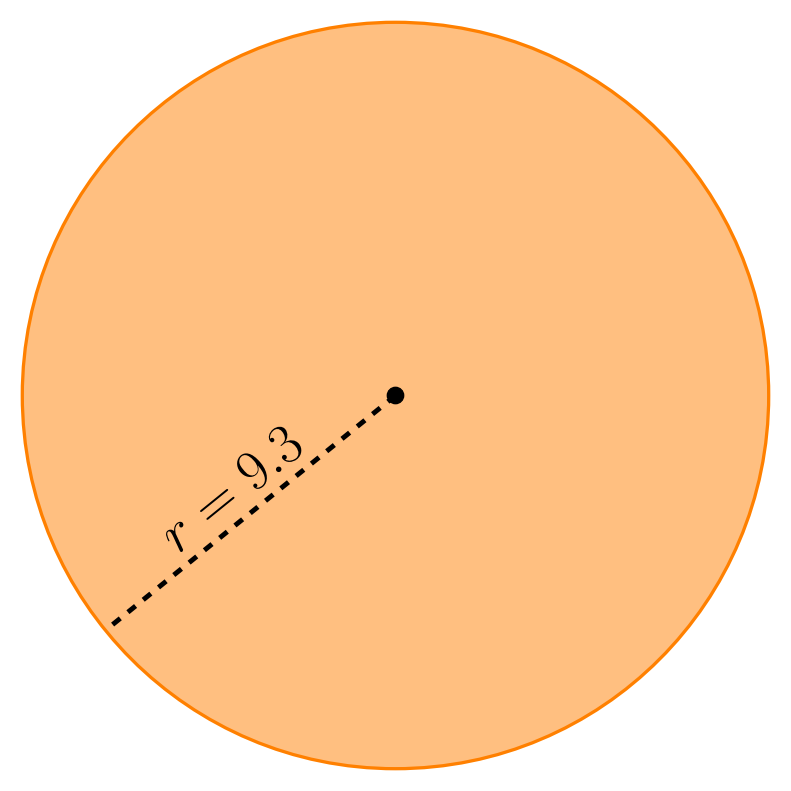
\includegraphics[width=0.8\linewidth]{../images/circulo06.png}\\
				\small Perímetro: \fillin[58.404][0.3in] Área: \fillin[271.57][0.3in]

				\begin{solutionbox}{1.2cm}\footnotesize
					% $P=2\pi r=2(3.14)(12)=75.36$ \\
					% $A=\pi r^2=3.14(12)^2=452.16$
				\end{solutionbox}
			\end{parts}
		\end{multicols}
	}

	% \addcontentsline{toc}{subsubsection}{Resolución de problemas}
	% \subsubsection*{Resolución de problemas}

	\addcontentsline{toc}{subsection}{Cuerpos Geométricos}
	\subsection*{Cuerpos Geométricos}
	% \addcontentsline{toc}{subsubsection}{Nombre de cuerpos geométricos}
	% \subsubsection*{Nombre de cuerpos geométricos}
	% \addcontentsline{toc}{subsubsection}{Elementos de cuerpos geométricos}
	% \subsubsection*{Elementos de cuerpos geométricos}
	% \addcontentsline{toc}{subsubsection}{Área lateral}
	% \subsubsection*{Área lateral}
	% \addcontentsline{toc}{subsubsection}{Área total}
	% \subsubsection*{Área total}
	% \addcontentsline{toc}{subsubsection}{Volumen}
	% \subsubsection*{Volumen}

	\addcontentsline{toc}{subsection}{Figuras Geométricas}
	\subsection*{Figuras Geométricas}
	% \addcontentsline{toc}{subsubsection}{Nombre de figuras}
	% \subsubsection*{Nombre de figuras}

	\questionboxed[2]{Escribe sobre la línea el nombre que recibe cada figura geométrica de acuerdo con su número de lados:

		\begin{multicols}{3}
			\begin{parts}
				\part 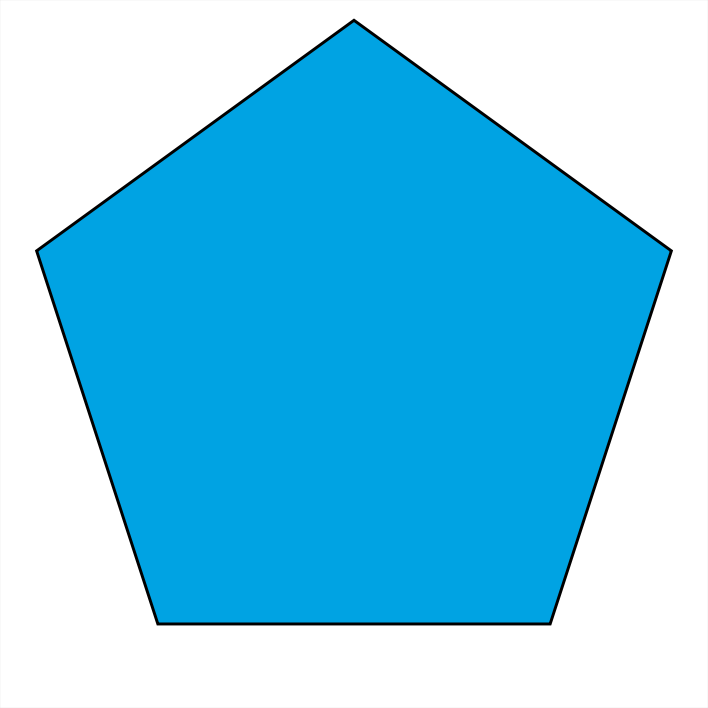
\includegraphics[width=75px]{../images/pentagono_azul.png}  \fillin[pentágono][0.75in]
				\part 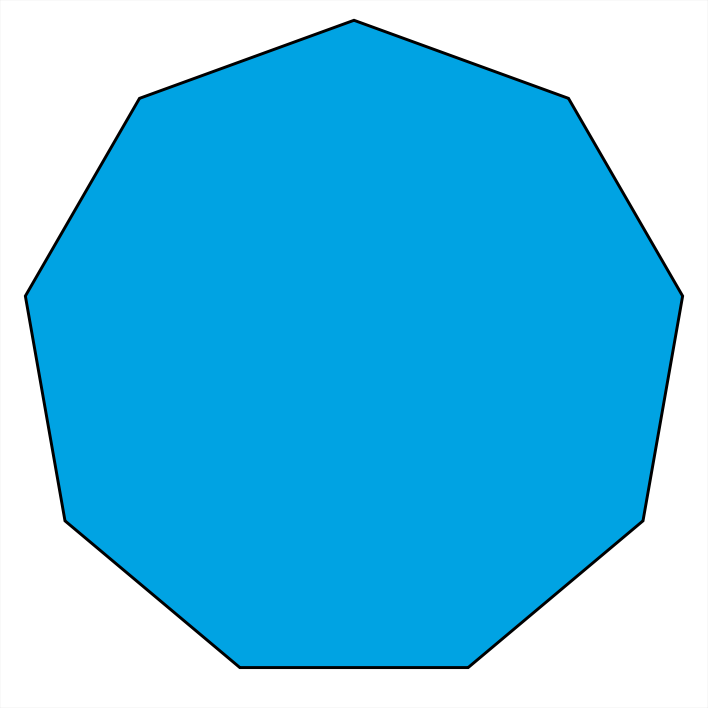
\includegraphics[width=75px]{../images/nonagono_azul.png}   \fillin[nonágono][0.75in]
				\part 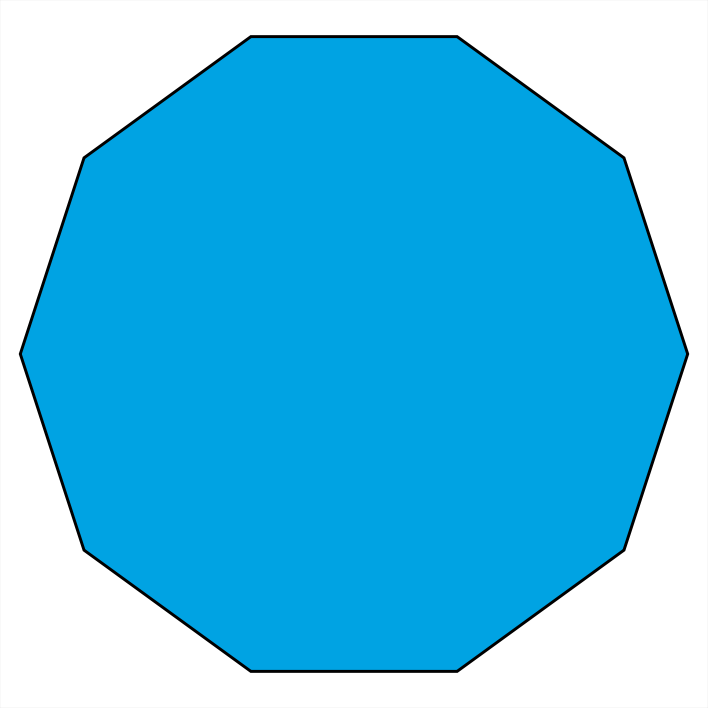
\includegraphics[width=75px]{../images/decagono_azul.png}   \fillin[decágono][0.75in]
				\part 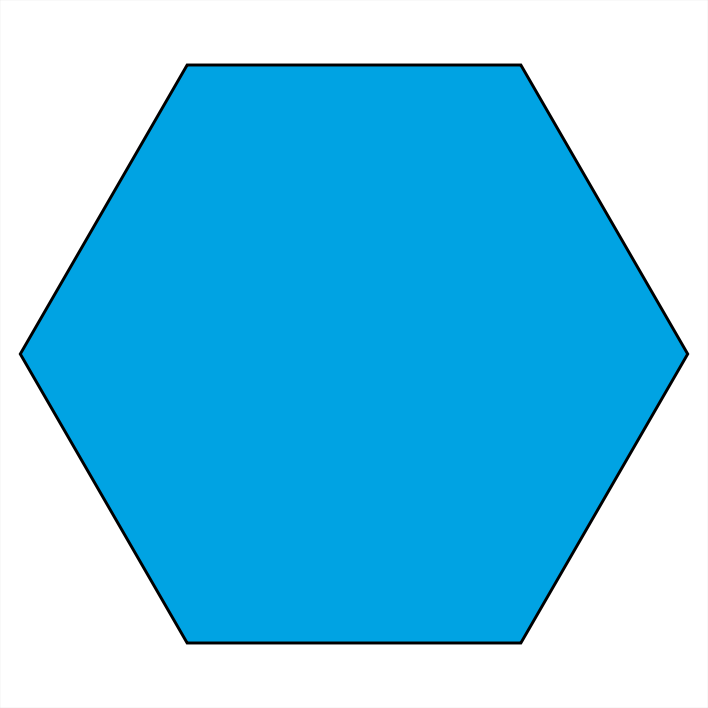
\includegraphics[width=75px]{../images/hexagono_azul.png}   \fillin[hexágono][0.75in]
				\part 
\includegraphics[width=75px]{../images/rectangulo_azul.png} \fillin[rectángulo][0.75in]
				\part 
\includegraphics[width=75px]{../images/cuadrado_azul.png}   \fillin[cuadrado][0.75in]
			\end{parts}
		\end{multicols}
	}

	% \addcontentsline{toc}{subsubsection}{Elementos de figuras}
	% \subsubsection*{Elementos de figuras}
	% \addcontentsline{toc}{subsubsection}{Perímetro}
	% \subsubsection*{Perímetro}

	\questionboxed[4]{Contesta las preguntas sobre perímetros de figuras geométricas

		\begin{multicols}{2}
			\begin{parts}
				\part ¿Cuál es el perímetro de un rectángulo cuya base mide 38 y su altura mide 19?

				\begin{solutionbox}{1cm}
					\[P=38+19+38+19=\color{red}114\]
				\end{solutionbox}

				\part ¿Cuál es el perímetro de un cuadrado que sus lados miden 5?

				\begin{solutionbox}{1cm}
					\[P=5+5+5+5=\color{red}20\]
				\end{solutionbox}

				\part ¿Cuál es el perímetro de un pentágono que sus lados miden 18?

				\begin{solutionbox}{1cm}
					\[P=18 \times 5=\color{red}90\]
				\end{solutionbox}

				% \part ¿Cuál es el perímetro de un octágono que sus lados miden 15?

				% \begin{solutionbox}{1cm}
				% 	\[P=15 \times 8=\color{red}120\]
				% \end{solutionbox}

				\part ¿Cuál es el perímetro de un rombo que sus lados miden 16?

				\begin{solutionbox}{1cm}
					\[P=16 \times 4=\color{red}64\]
				\end{solutionbox}

			\end{parts}
		\end{multicols}
	}

	% \addcontentsline{toc}{subsubsection}{Área}
	% \subsubsection*{Área}

	\questionboxed[2]{Contesta las preguntas sobre áreas de figuras geométricas

		\begin{multicols}{2}
			\begin{parts}
				\part ¿Cuál es el área de un triángulo cuya base mide 18 y su altura mide 11?

				\begin{solutionbox}{1.5cm}
					\[A=\dfrac{18 \times 11}{2}=\color{red}99\]
				\end{solutionbox}


				\part ¿Cuál es el área de un cuadrado que sus lados miden 29?

				\begin{solutionbox}{1.5cm}
					\[A=29 \times 29=\color{red}841\]
				\end{solutionbox}

			\end{parts}
		\end{multicols}
	}

	% \addcontentsline{toc}{subsubsection}{}
	% \subsubsection*{Resolución de problemas}

	\questionboxed[2]{
		\begin{multicols}{2}
			\begin{parts}
				\part Convierte 23 horas a minutos:    \begin{solutionbox}{1cm}\fillin[1380][0in]\end{solutionbox}
				\part Convierte 27 horas a segundos:   \begin{solutionbox}{1cm}\fillin[97200][0in]\end{solutionbox}
				\part Convierte 3.9 horas a minutos:   \begin{solutionbox}{1cm}\fillin[234][0in]\end{solutionbox}
				\part Convierte 4.8 minutos a segundos:\begin{solutionbox}{1cm}\fillin[288][0in]\end{solutionbox}
			\end{parts}
		\end{multicols}
	}

	\addcontentsline{toc}{subsection}{Sistema de Unidades}
	\subsection*{Sistema de Unidades}
	% \addcontentsline{toc}{subsubsection}{Operaciones con múltiplos de 10}
	% \subsubsection*{Operaciones con múltiplos de 10}
	% \addcontentsline{toc}{subsubsection}{Unidades de longitud}
	% \subsubsection*{Unidades de longitud}
	% \addcontentsline{toc}{subsubsection}{Unidades de masa}
	% \subsubsection*{Unidades de masa}
	% \addcontentsline{toc}{subsubsection}{Unidades de capacidad}
	% \subsubsection*{Unidades de capacidad}
	% \addcontentsline{toc}{subsubsection}{Unidades de área y volumen}
	% \subsubsection*{Unidades de área y volumen}


\end{questions}
\end{document}